\documentclass[UTF8,a4paper,11pt,openany,fontset=fandol]{ctexbook}
\usepackage[a4paper,margin=23mm,headheight=15pt]{geometry}
\usepackage{amsmath,amssymb,bm,mathtools,booktabs,longtable,tabularx,array,graphicx}
\usepackage{enumitem,xcolor,fancyhdr,needspace}
\usepackage[numbers,sort&compress]{natbib}
\usepackage{float}
\usepackage{hyperref,bookmark}
\usepackage{tikz}
\usetikzlibrary{arrows.meta,positioning}
\setCJKmainfont{FandolSong-Regular.otf}[BoldFont=FandolSong-Bold.otf,ItalicFont=FandolKai-Regular.otf]
\setCJKsansfont{FandolHei-Regular.otf}[BoldFont=FandolHei-Bold.otf]
\setCJKmonofont{FandolFang-Regular.otf}
\setmainfont{texgyretermes-regular.otf}[BoldFont=texgyretermes-bold.otf,ItalicFont=texgyretermes-italic.otf,BoldItalicFont=texgyretermes-bolditalic.otf]\setsansfont{texgyreheros-regular.otf}[BoldFont=texgyreheros-bold.otf]
\definecolor{ink}{HTML}{193D55}
\ctexset{chapter={format=\sffamily\huge\bfseries\color{ink},beforeskip=0pt,afterskip=20pt},section={format=\sffamily\Large\bfseries\color{ink}},subsection={format=\sffamily\large\bfseries},subsubsection={format=\sffamily\normalsize\bfseries}}
\hypersetup{colorlinks=true,linkcolor=ink,citecolor=ink,urlcolor=ink,bookmarksnumbered=true,bookmarksdepth=2,pdftitle={Hall MHD与双流体磁重联：模型推导、数值方法与文献调研}}
\setlength{\emergencystretch}{4em}\setlength{\parskip}{3pt}\linespread{1.12}\raggedbottom
\setlist{nosep,leftmargin=2em}\setcounter{tocdepth}{1}\setcounter{secnumdepth}{2}
\pagestyle{fancy}\fancyhf{}\fancyhead[L]{\small\nouppercase{\leftmark}}\fancyfoot[C]{\thepage}
\newcommand{\vct}[1]{\bm{#1}}\newcommand{\dd}{\mathrm d}\newcommand{\VA}{V_{\!A}}\newcommand{\J}{\vct J}\newcommand{\B}{\vct B}\newcommand{\E}{\vct E}\newcommand{\vel}{\vct u}\newcommand{\grad}{\nabla}\newcommand{\R}{\mathcal R}
\newcommand{\note}[1]{\par\smallskip\noindent\textsf{\textbf{学习提示：}}#1\par\smallskip}
\newcommand{\assume}[1]{\par\smallskip\noindent\textsf{\textbf{假设与边界：}}#1\par\smallskip}
\newcolumntype{P}[1]{>{\raggedright\arraybackslash}p{#1}}
\numberwithin{equation}{chapter}

\let\cleardoublepage\clearpage

\tracinglostchars=3
\usetikzlibrary{calc,decorations.pathreplacing,shapes.geometric}
\newcommand{\worked}[1]{\par\medskip\noindent\textsf{\textbf{完整算例：#1}}\par\smallskip}
\newcommand{\Deta}{D_\eta}
\renewcommand{\theequation}{\thechapter.\arabic{equation}}

\hypersetup{pdftitle={从等离子体导论到双流体与Hall MHD：磁重联讲义}}
\begin{document}\frontmatter
\begin{titlepage}
\vspace*{20mm}
{\sffamily\Large 磁场重联 · 研究生入门讲义\par}
\vspace{15mm}
{\sffamily\Huge\bfseries\color{ink}从等离子体导论\\[8pt]到双流体与 Hall MHD\par}
\vspace{14mm}
{\Large 方程怎样来，近似怎样选，数字怎样算\par}
\vspace{12mm}
{\large 逐步理论推导 · 完整数值算例 · 原创解析配图\par}
\vfill
编写日期：2026年11月16日。\\[8pt]
阅读前提：学过等离子体导论，知道洛伦兹力、Maxwell方程、回旋运动及Debye屏蔽；不要求已学过磁重联或张量流体理论。\\[8pt]
本讲义独立可读。公式按定义、推导、近似和适用条件展开；教学输入与文献实测分别标识。配图由附带脚本绘制；未宣称运行或复现大型重联模拟。
\end{titlepage}
\chapter*{怎样使用这份讲义}
不要第一次就试图记住全部欧姆定律。第一遍先建立“粒子分布—矩方程—闭合—约化—重联层”这条主线；第二遍亲自代入第7章的数字，体会同一系统的大尺度与薄层为什么需要不同模型；第三遍检查第11章的完整解答，并带着第10章的问题阅读原始论文。

本讲义将所有必要变量在使用前定义，明确电子电荷的负号、温度单位、压力张量与热流阶数。加框公式标出重要结果，紧邻文字说明其条件。图中的解析曲线和示意图不冒充实验或模拟数据。文献引用用于注明既有模型和观测来源；本次教学整理不增加原调研库的全文核读计数。

伴随讲义Lecture-TM进一步讲解撕裂模：从电流片的线性不稳定性到磁岛非线性增长和实验诊断。两份讲义采用不同的常见二维坐标约定，已在各自开头说明；先核对定义再比较分量公式。
\setcounter{tocdepth}{1}\tableofcontents\listoffigures
\mainmatter
\chapter{从导论课走向磁重联：先建立一张可计算的地图}
\label{hall:orientation}
\section{这份讲义要让你真正会做什么}
导论课已经告诉我们：带电粒子受洛伦兹力，粒子会回旋，等离子体能够屏蔽电场，也能支持各种波。现在的问题是：数以亿计的粒子共同形成一层很薄的电流片时，磁场为什么会改变连接方式？离子与电子是否仍能被看成一团共同运动的物质？哪条方程告诉我们模型失效了？

本讲义把这些问题转成五项可练习的能力：能从分布函数推导物种方程；能说明每次约化删掉了哪项和为什么能删；能用实际数字比较欧姆定律各项；能从磁通、能量和尺度判断某个重联图像是否自洽；能看懂一篇Hall或双流体论文究竟求解了什么。所有主要数量级例题均给出计算过程和结论，不把关键步骤留给读者补。

\note{第一次阅读可以先读本章，然后连续读第2--5章掌握方程来源；第7章的数字算例应逐行跟算。第8章把方程放回重联层，第9章用波检验Hall项，第10章讨论模拟与证据。第11章含有完整答案，用来检查是否真正掌握。}

\section{同一等离子体的三个描述层次}
\paragraph{粒子层次。}每个电子都服从$m_e\dd\vct v/\dd t=-e(\E+\vct v\times\B)$。若直接跟踪全部真实粒子，变量太多；粒子模拟也只是以数值粒子抽样分布。
\paragraph{分布函数层次。}$f_s(\vct x,\vct v,t)\dd^3x\dd^3v$表示位置和速度小体积中的粒子数。它能区分向右运动的一束和向左运动的一束，即使两束的平均速度为零。
\paragraph{流体层次。}把速度空间积分，得到密度、平均速度、压力及热流。电子是一套，离子是一套，便是本文的\emph{电子--离子双流体}。双流体并不是两种互不相干的液体：两者通过同一电磁场和碰撞强烈耦合。

理想MHD进一步以近似共同的整体运动描述两者。Hall MHD则保留电子和离子之间对磁通输运重要的相对运动。它常写成一套总动量方程加一条广义欧姆定律，外观像单流体，但仍含两物种的差异。因此“方程里只有一个显式速度演化式”不能用来判断是否保留了双流体物理。

\section{单位、温度和坐标：先约定，后计算}
全文采用SI单位。$e=1.602176634\times10^{-19}\,\mathrm C$是\emph{正}的元电荷，离子电荷$+e$，电子电荷$-e$。默认离子为质子，质量$m_i=1.67262\times10^{-27}\,\mathrm{kg}$；电子质量$m_e=9.10938\times10^{-31}\,\mathrm{kg}$。氘或多电荷离子需要重新代入质量与电荷，不能沿用所有氢的数值。

用$\Theta_s=k_BT_{s,\mathrm K}$表示以焦耳为单位的温度能量，故标量压强$p_s=n_s\Theta_s$。若实验写$T_s=20\,\mathrm{eV}$，计算时用
\begin{equation}
\Theta_s=e\,(20\,\mathrm V)=3.20435\times10^{-18}\,\mathrm J,
\end{equation}
通常简写为$\Theta_s=eT_s$，这里$T_s$指以eV报告的数值。不要再乘一次$k_B$。热速度约定为$v_{ts}=\sqrt{2\Theta_s/m_s}$；有些教材用不含2的定义，所以比较回旋半径和碰撞平均自由程前应先对齐约定。

电阻率写$\eta$，单位$\Omega\,\mathrm m$；磁扩散系数写$D_\eta=\eta/\mu_0$，单位$\mathrm{m^2/s}$。文献常把两者都叫$\eta$，但本讲义不混用。$\Omega_s$是角频率，单位$\mathrm{s^{-1}}$；普通频率$f_s=|\Omega_s|/(2\pi)$，二者不能少除一个$2\pi$。

二维重联采用$x$为出流方向、$y$为入流方向、$z$为面外电流/导场方向。图\ref{hall:figgeometry}中的磁力线是解析示意，不是模拟或实测。伴随讲义Lecture-TM采用另一常见约定$x$跨片、$y$沿片；两份讲义的物理相同，但不要直接照搬分量下标。
\begin{figure}[htbp]\centering
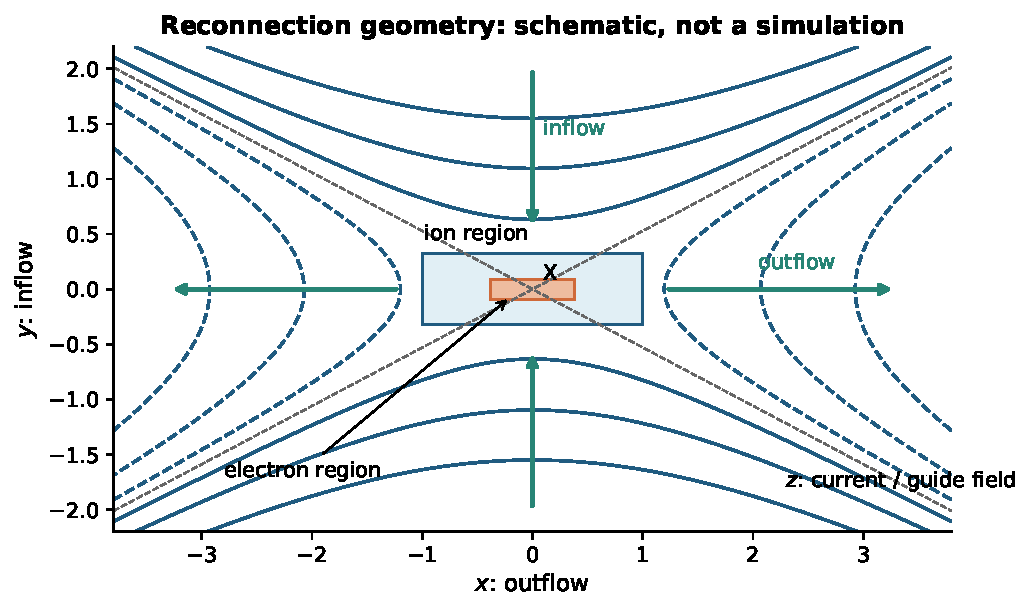
\includegraphics[width=.94\textwidth]{figures/01_geometry.pdf}
\caption{重联几何及两个内层的示意。蓝色等值线来自$A_z=(y^2-0.28x^2)/2$；矩形仅表示尺度层次，不表示真实层宽或层长比。绿色箭头为入流与出流，真实解须同时满足连续性、动量和磁通约束。}\label{hall:figgeometry}
\end{figure}

\section{磁力线、磁通与“断线”分别指什么}
磁力线是在\emph{同一时刻}处处与$\B$相切的曲线，满足$\dd\vct x/\dd l\parallel\B$；它不是一根有材料编号的橡皮绳。所谓磁场连接关系，是场线从一个区域进入、沿磁场到达哪个区域的映射。重联讨论这个映射怎样随时间改变，而不是用肉眼判断两条线是否在画面上相交。

二维$\partial_z=0$时可写
\begin{equation}
\B_\perp=\nabla A_z\times\hat{\vct z}
=(\partial_yA_z,-\partial_xA_z,0),\qquad
\B_\perp\cdot\nabla A_z=0.
\end{equation}
所以$A_z$的等值线就是面内磁力线。相邻等值线的$\Delta A_z$表示单位$z$长度的磁通，单位是$\mathrm{T\,m= Wb/m}$。它不是磁场强度，量纲比$B$多一个长度。

X点是$A_z$的鞍点：两个方向曲率符号相反；O点是局地极大或极小点，周围有闭合等值线形成磁岛。分离线经过X点，区分不同连接区域。三维里没有一个标量$A_z$能替代全部场线拓扑；不能把二维X点公式不加说明地直接套到三维。

\section{一个电流片为什么能够静止：Harris型力平衡}
先不谈重联，构造静态平衡。设
\begin{equation}
\B=B_x(y)\hat{\vct x}+B_g\hat{\vct z},\qquad B_x=B_0\tanh(y/a),
\end{equation}
$a$为半厚度，$B_g$为常数导场。忽略位移电流，逐分量求旋度：
\begin{equation}
\J=\frac{\nabla\times\B}{\mu_0}
=-\frac{B_0}{\mu_0a}\operatorname{sech}^2(y/a)\hat{\vct z}.
\end{equation}
由于$\hat{\vct z}\times\hat{\vct x}=\hat{\vct y}$，洛伦兹力的$y$分量为$J_zB_x=-B_x\partial_yB_x/\mu_0$。静态总动量平衡$0=-\nabla p+\J\times\B$给
\begin{align}
\frac{\dd p}{\dd y}&=-\frac{B_x}{\mu_0}\frac{\dd B_x}{\dd y},\\
\frac{\dd}{\dd y}\left(p+\frac{B_x^2}{2\mu_0}\right)&=0,\\
p(y)&=p_\infty+\frac{B_0^2}{2\mu_0}\operatorname{sech}^2(y/a).
\end{align}
导场为常数，其磁压也为常数，因此不出现在梯度中。电流片中间反向磁场减弱，总热压必须增加以补偿。这个压力可以由更高密度、更高温度或二者共同提供，不能只凭平衡式唯一决定。
\begin{figure}[htbp]\centering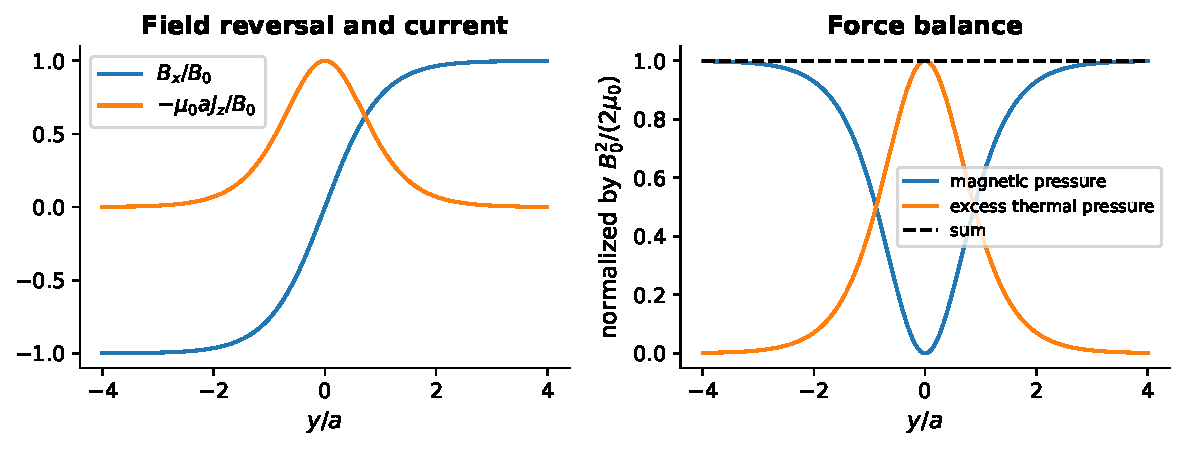
\includegraphics[width=\textwidth]{figures/02_harris.pdf}
\caption{Harris型平衡的解析曲线。左图电流取负号后与$\operatorname{sech}^2$同号；右图显示增加的热压与反向磁场的磁压之和恒定。此图检验静态力平衡，不表示重联已经发生。}\label{hall:figharris}\end{figure}

\worked{已算例：电流并不要求大量电荷分离}
取$B_0=0.05\,\mathrm T$、$a=0.01\,\mathrm m$、中心密度$n=10^{19}\,\mathrm{m^{-3}}$。中心电流绝对值
\begin{equation}
|J_z(0)|=\frac{0.05}{(1.25664\times10^{-6})(0.01)}
=3.98\times10^6\,\mathrm{A/m^2}.
\end{equation}
即使$n_i=n_e=n$，仍有
\begin{equation}
|u_{iz}-u_{ez}|=\frac{|J_z|}{en}
=\frac{3.98\times10^6}{(1.60218\times10^{-19})(10^{19})}
=2.48\times10^6\,\mathrm{m/s}.
\end{equation}
电荷密度$e(n_i-n_e)$为零，而电流不为零，因为电子和离子的\emph{通量}不同。本例只给了总流差；由电子承担多少，需要额外初始条件。若把它全部分配给电子，应另外检查其漂移能和可能的流致不稳定性。

\section{一张模型选择表，以及两个需要避免的误解}
\begin{longtable}{P{25mm}P{51mm}P{70mm}}
\toprule 模型 & 保留的主要信息 & 一开始就该问的问题\\\midrule\endfirsthead
\toprule 模型 & 保留的主要信息 & 一开始就该问的问题\\\midrule\endhead
理想MHD & 总体流动，理想磁通冻结 & 目标层厚是否远大于非MHD尺度？是否需要改变磁连接？\\
电阻MHD & 总体运动与电阻磁扩散 & 电阻来自什么碰撞/模型？层内是否仍适用流体闭合？\\
Hall MHD & 离子/总体流与电子磁通输运不同 & 电子层由什么破冻结？电子压强及热流怎样闭合？\\
惯性扩展 & 增加电子惯性/相对流能 & 保留的惯性与总能量是否一致？是否使用准中性？\\
五矩双流体 & 两套密度、动量、标量能量 & 是否需要各向异性/非对角压力？电磁方程取何约化？\\
十矩双流体 & 两套对称压力张量 & 三阶热流怎么关？压力是否正定，闭合有无校准依赖？\\
\bottomrule\end{longtable}
“双流体”是物种划分，“五矩/十矩”是保留的速度矩阶数，“准中性/全Maxwell”是电磁约化；它们不是同一条线上的互斥选项。第二个误解是“更复杂一定更准确”。复杂方程若闭合、边界或网格不合适，也会给出错误温度和电场。我们将反复区分数学上\emph{能表示}一个量、数值上\emph{算得收敛}和物理上\emph{通过观测}这三件事。\citep{Birn2001,Wang2015}

\chapter{从分布函数到流体：逐项推导矩方程}
\label{hall:sec:moments}
\section*{读这一章要解决什么}
导论课程常直接给出流体连续性和动量方程。本章把它们从粒子分布重新推出来，目的是让你知道每个项的来源，尤其是为什么压力会成为张量、为什么还需要热流，以及为什么“把粒子平均”没有自动完成闭合。
本章先用物种下标$s$推一次共同数学结构，下一章将离子和电子分别列全。$q_i=+e$、$q_e=-e$，$e>0$；不要将标量电荷$q_s$与粗体热流$\vct q_s$混淆。空间分量用$i,j,k$；写$P_{s,ij}$时，逗号前是物种，逗号后是分量。

约定温度能量$\Theta_s=k_BT_{s,\mathrm K}$，单位J，若实验温度用eV报告为$T_{s,\mathrm{eV}}$，则$\Theta_s=eT_{s,\mathrm{eV}}$。这里数值“$T_{s,\mathrm{eV}}=100$”表示100 eV，而不是100 J。标量温度定义为$\Theta_s=p_s/n_s$。这一定义即使对非Maxwell分布也能使用，但其意义首先是二阶矩，不保证代表单一热核心。

\section{分布函数不是流速；先明确积分在什么空间进行}
$f_s(\vct x,\vct v,t)\dd^3x\dd^3v$表示相空间小体积内的粒子数。固定位置$\vct x$后，对$\vct v$积分才得到该位置的数密度；同一点可以同时存在向相反方向运动的粒子。没有碰撞时也仍然可以定义平均流与压力。

非相对论Vlasov--Boltzmann方程是
\begin{equation}
 \partial_tf_s+v_j\partial_jf_s+
 \frac{q_s}{m_s}(E_j+\epsilon_{jkl}v_kB_l)\partial_{v_j}f_s=C_s[f].
 \label{hall:eq:vlasov}
\end{equation}
左边依次是在固定相空间点的时间变化、粒子在真实空间的运动、Lorentz力造成的速度空间运动。右边$C_s$表示碰撞；需要电离、复合时还应增加相应源项。本节暂时假设每个物种粒子数守恒，即$\int C_s\dd^3v=0$。
\begin{align}
 n_s&=\int f_s\dd^3v,&
 n_s\vct u_s&=\int\vct v f_s\dd^3v,\\
 \vct c&=\vct v-\vct u_s,&
 \int\vct c f_s\dd^3v&=0,\\
 P_{s,ij}&=m_s\int c_ic_j f_s\dd^3v,&
 Q_{s,ijk}&=m_s\int c_ic_jc_k f_s\dd^3v,\\
 p_s&=\frac13P_{s,ii},&
 q_{s,k}&=\frac12Q_{s,iik}.
\end{align}
其中$\rho_s=m_sn_s$。$\mathsf P_s$描述围绕平均流的随机运动；冷粒子束即使整体流速很大，相对于其自身平均速度的压力仍可以很小。反过来，两束方向相反的冷束总平均速度为零，总压力却不为零。

\section{所有矩方程共同使用的一次分部积分}
记加速度$a_j=(q_s/m_s)(E_j+\epsilon_{jkl}v_kB_l)$。由于场不依赖粒子速度，
\begin{equation}
 \partial_{v_j}a_j=\frac{q_s}{m_s}\epsilon_{jkl}\delta_{jk}B_l=0.
\end{equation}
对只依赖$\vct v$的权函数$w(\vct v)$，在速度空间半径$R$的球内先积分：
\begin{equation}
 \int w a_j\partial_{v_j}f_s\dd^3v
 =\oint_{|\vct v|=R}w f_s\vct a\cdot\dd\vct S_v
 -\int f_s a_j\partial_{v_j}w\dd^3v.
\end{equation}
若$f_s$衰减得足够快，使所考虑阶矩及表面通量收敛，令$R\to\infty$后表面项消失。将剩下的负项移到方程右边：
\begin{equation}
 \partial_t\int wf_s\dd^3v+\partial_j\int v_jwf_s\dd^3v
 =\int f_s\vct a\cdot\grad_vw\,\dd^3v+\int wC_s\dd^3v.
 \label{hall:eq:tutorial-mastermoment}
\end{equation}
这就是取矩的通用公式。若选$w=m_sc_ic_j$，由于$\vct u_s(\vct x,t)$也在$c_i$中，权函数额外依赖时空，不能直接套用这个简化式。因此下面先取原始矩$v_iv_j$，再减去平均运动，步骤更不容易出错。

\section{零阶矩：把每一项都写出来}
取$w=1$。时间项给$\partial_t n_s$，空间通量给$\partial_j(n_su_{s,j})$，而$\grad_vw=0$使力项为零。粒子数守恒的碰撞积分也为零，于是
\begin{equation}
 \partial_tn_s+\grad\cdot(n_s\vct u_s)=0.
 \label{hall:eq:continuity}
\end{equation}
展开散度：
\begin{equation}
 \partial_t n_s+\vct u_s\cdot\grad n_s+n_s\grad\cdot\vct u_s=0
 \quad\Longrightarrow\quad
 D_sn_s=-n_s\theta_s,\quad\theta_s=\grad\cdot\vct u_s.
\end{equation}
正散度表示小流体团膨胀，密度随之降低。这个方程并没有要求麦克斯韦分布、压强各向同性、低温或无碰撞。

\paragraph{跟算例：均匀膨胀。}
令$\vct u=a(t)\vct x$，则$\theta=3a$。沿流轨迹有
$n(t)=n(0)\exp[-3\int_0^ta(t')\dd t']$。如果空间只允许二维变化，但取$u_z=0$，则该特定流的散度是$2a$；这与速度分布仍有三个自由度并不冲突。

\section{一阶矩：电磁力的符号从哪里来}
对第$i$个分量取$w=m_sv_i$。由$\partial_{v_j}w=m_s\delta_{ij}$，
\begin{align}
 \int f_s\vct a\cdot\grad_vw\,\dd^3v
 &=q_s\int f_s(E_i+\epsilon_{ikl}v_kB_l)\dd^3v\\
 &=q_sn_s(E_i+\epsilon_{ikl}u_{s,k}B_l).
\end{align}
电子的$q_e=-e$在这一步保留；不应在得到欧姆定律后凭直觉补符号。
再展开动量通量中的乘积：
\begin{align}
 m_s\int v_iv_jf_s\dd^3v
 &=m_s\int(u_i+c_i)(u_j+c_j)f_s\dd^3v\\
 &=\rho_su_iu_j+
 m_su_i\int c_jf_s\dd^3v+
 m_su_j\int c_if_s\dd^3v+
 m_s\int c_ic_jf_s\dd^3v\\
 &=\rho_su_iu_j+P_{s,ij}.
\end{align}
两个交叉项严格为零，使用的是平均速度的定义。定义碰撞动量交换$\vct R_s=m_s\int\vct vC_s\dd^3v$，得到
\begin{equation}
 \partial_t(\rho_s\vct u_s)+
 \grad\cdot(\rho_s\vct u_s\vct u_s+\mathsf P_s)
 =q_sn_s(\E+\vct u_s\times\B)+\vct R_s.
 \label{hall:eq:momentum}
\end{equation}
现在才把它变成随体形式。以$x$分量为例，
\begin{align}
 \partial_t(\rho u_x)+\partial_j(\rho u_ju_x)
 &=\rho\partial_tu_x+\rho u_j\partial_ju_x
   +u_x[\partial_t\rho+\partial_j(\rho u_j)]\\
 &=\rho Du_x.
\end{align}
三个分量合起来即
\begin{equation}
 \rho_sD_s\vct u_s=q_sn_s(\E+\vct u_s\times\B)
                  -\grad\cdot\mathsf P_s+\vct R_s.
 \label{hall:eq:speciesmom}
\end{equation}
左边的量纲是$ {\rm kg\,m^{-3}}\times{\rm m\,s^{-2}}={\rm N\,m^{-3}}$，右边每一项也必须是单位体积的力。压力沿$x$增大时$-\partial_xp<0$，流体受到指向低压侧的力，可用来检查符号。

\section{二阶原始矩：八项乘积不能省略成一句话}
暂省物种下标。定义
$M_{ij}=m\int v_iv_jf\dd^3v=\rho u_iu_j+P_{ij}$。
取$w=mv_iv_j$时
$\partial_{v_l}w=m(\delta_{il}v_j+\delta_{jl}v_i)$，所以
\begin{align}
 \partial_tM_{ij}+\partial_k\mathcal Q_{ijk}
 &=qn(E_iu_j+E_ju_i)\\
 &\quad+\frac qm
 (\epsilon_{ikl}M_{kj}B_l+\epsilon_{jkl}M_{ki}B_l)
 +\mathcal C^{(2)}_{ij},\nonumber
\end{align}
其中$\mathcal C^{(2)}_{ij}=m\int v_iv_jC\dd^3v$。空间通量需要三阶原始矩，逐项展开
\begin{align}
 v_iv_jv_k={}&u_iu_ju_k
 +c_iu_ju_k+u_ic_ju_k+u_iu_jc_k\\
 &+u_ic_jc_k+c_iu_jc_k+c_ic_ju_k+c_ic_jc_k.\nonumber
\end{align}
积分后，含一个$c$的三项为零，含两个$c$的三项留下压力，因此
\begin{equation}
 \mathcal Q_{ijk}
 =\rho u_iu_ju_k+u_iP_{jk}+u_jP_{ik}+u_kP_{ij}+Q_{ijk}.
 \label{hall:eq:tutorial-rawthird}
\end{equation}
到此仍没有闭合：右侧最后一个$Q_{ijk}$是新的未知量。

\section{减去平均动能：压力方程中的电场为何消失}
用连续性和乘积法则得到
\begin{equation}
 \partial_t(\rho u_iu_j)+\partial_k(\rho u_iu_ju_k)
 =\rho u_iDu_j+\rho u_jDu_i.
\end{equation}
把动量方程代入右边，其中电场部分恰为$qn(u_iE_j+u_jE_i)$；磁场的平均流部分恰为
$(q/m)(\epsilon_{ikl}\rho u_ku_jB_l+\epsilon_{jkl}\rho u_ku_iB_l)$。
它们分别与二阶原始矩的对应部分抵消。
还要处理压力乘积。例如
\begin{equation}
 \partial_k(u_iP_{jk})-u_i\partial_kP_{jk}
 =P_{jk}\partial_ku_i.
\end{equation}
另一项同理。剩下的$u_kP_{ij}$不作消去，保留成压力的对流通量。于是
\begin{align}
 \partial_tP_{ij}+\partial_k(u_kP_{ij})
 +P_{ik}\partial_ku_j+P_{jk}\partial_ku_i+\partial_kQ_{ijk}
 ={}&\frac qm(\epsilon_{ikl}P_{kj}B_l+\epsilon_{jkl}P_{ki}B_l)
 +C_{ij}.
 \label{hall:eq:pressure}
\end{align}
这里$C_{ij}=m\int c_ic_jC\dd^3v$。在粒子数守恒时，它等于$\mathcal C^{(2)}_{ij}-u_iR_j-u_jR_i$；因此碰撞引起的整体加速与随机能量变化已经分开。

这条式子右边没有显式电场，不表示电场不能间接改变温度。电场先改变平均流，流的空间梯度再通过左侧两个压力应变项改变随机运动。热流把邻近位置的速度分布信息带入本地。

\paragraph{跟算例：均匀磁场只旋转压力椭球。}
取$\vct u=0$、空间均匀、$\B=B_0\hat z$、$Q=C=0$，记带符号回旋频率$\Omega=qB_0/m$。压力方程逐分量变为
\begin{align}
 \dot P_{xx}&=2\Omega P_{xy},&
 \dot P_{yy}&=-2\Omega P_{xy},&
 \dot P_{zz}&=0,\\
 \dot P_{xy}&=\Omega(P_{yy}-P_{xx}),&
 \dot P_{xz}&=\Omega P_{yz},&
 \dot P_{yz}&=-\Omega P_{xz}.
\end{align}
前三式相加立刻得到$\partial_t\operatorname{tr}\mathsf P=0$。磁场可以改变非对角压力，却不能通过这一旋转项增加总随机能量。电子的$\Omega<0$，旋转方向相反。

\section{取迹得到内能：解释每一个二分之一}
随机平动能密度为
\begin{equation}
 U_s=\frac{m_s}2\int c^2f_s\dd^3v=\frac12P_{s,ii}.
\end{equation}
令压力方程$i=j$并求和。两个压力应变项相同，相加为$2P_{ik}\partial_ku_i$；磁旋转项为零，因为对称的$P_{ik}$与反对称的$\epsilon_{ikl}$缩并为零。定义$q_k=Q_{iik}/2$、$H_s=C_{s,ii}/2$，全式除以2：
\begin{equation}
 \partial_tU_s+\grad\cdot(U_s\vct u_s)
 +\mathsf P_s:\grad\vct u_s+\grad\cdot\vct q_s=H_s.
 \label{hall:eq:internal}
\end{equation}
如果$\mathsf P=p\mathsf I$，则$U=3p/2$且$\mathsf P:\grad\vct u=p\theta$。压缩时$\theta<0$，右移后的$-p\theta$为正，表示压缩做功增加内能。压力应变在无碰撞演化中可以反向，不能自动称为不可逆热化。

\section{再把平均流能加回来，检查电磁功的去向}
定义$K_s=\rho_su_s^2/2$。动量方程点乘$\vct u_s$，并用
\begin{equation}
 \vct u_s\cdot(\grad\cdot\mathsf P_s)
 =\grad\cdot(\mathsf P_s\cdot\vct u_s)-\mathsf P_s:\grad\vct u_s
\end{equation}
得到
\begin{equation}
 \partial_tK_s+\grad\cdot(K_s\vct u_s+\mathsf P_s\cdot\vct u_s)
 =q_sn_s\vct u_s\cdot\E+\mathsf P_s:\grad\vct u_s+\vct u_s\cdot\vct R_s.
\end{equation}
这里$\vct u_s\cdot(\vct u_s\times\B)=0$。与内能方程相加，压力应变一正一负抵消：
\begin{equation}
 \partial_t\mathcal E_s+
 \grad\cdot(\mathcal E_s\vct u_s+\mathsf P_s\cdot\vct u_s+\vct q_s)
 =q_sn_s\vct u_s\cdot\E+\vct u_s\cdot\vct R_s+H_s,
 \quad\mathcal E_s=K_s+U_s.
 \label{hall:eq:energy}
\end{equation}
所以压力应变是平均流能与内能之间的交换；电磁功连接场能与粒子总能。只有把这几条方程同时列出，才能准确判断模拟图中的“能量转换”是哪一个通道。

\section{为什么有了这些精确方程仍然没有求解完整问题}
密度方程含速度，动量方程含压力，压力方程含三阶矩；继续取三阶矩又会出现四阶矩。精确取矩没有减少所需信息，只是重新组织信息。设定$Q=0$、设定$\mathsf P=p\mathsf I$、采用Landau型热流，都是额外物理近似，不能由积分运算自动得到。

\paragraph{自检与答案。}
若两个等密度冷电子束分别以$\pm V\hat x$运动，总数密度为$n$，则$\vct u=0$，$P_{xx}=mnV^2$，$P_{yy}=P_{zz}=0$，$p=mnV^2/3$。若此时强行改成$p\mathsf I$，总内能$3p/2$不变，但沿$x$的应力从$mnV^2$变成$mnV^2/3$，另外两个方向凭空出现压力。这说明“内能相同”不能保证重联喷流和压力支撑相同。五矩与十矩的区别正从这里开始。\citep{Wang2015,Ng2020}

\section{用一个明确的分布检查“流速”和“温度”}
考虑某一方向的两个窄束；每束密度$n/2$、相对各自中心的热速度方差$\sigma^2$，中心速度为$+V$与$-V$。总分布的一维形式为
\begin{equation}
f_x(v_x)=\frac{n}{2\sqrt{2\pi}\sigma}
\left[\exp\!\left(-\frac{(v_x-V)^2}{2\sigma^2}\right)
+\exp\!\left(-\frac{(v_x+V)^2}{2\sigma^2}\right)\right].
\end{equation}
对第一个高斯令$w=v_x-V$，对第二个令$w=v_x+V$。奇函数积分给$\int w\exp[-w^2/(2\sigma^2)]\dd w=0$，于是
\begin{align}
 u_x&=\frac1n\left(\frac n2V-\frac n2V\right)=0,\\
 P_{xx}&=m\int v_x^2f_x\dd v_x
 =\frac{mn}{2}(V^2+\sigma^2)+\frac{mn}{2}(V^2+\sigma^2)
 =mn(V^2+\sigma^2).
\end{align}
若另两方向各有同样的束内方差，则$P_{yy}=P_{zz}=mn\sigma^2$，而
\begin{equation}
\Theta=\frac{P_{xx}+P_{yy}+P_{zz}}{3n}
 =m\sigma^2+\frac13mV^2.
\end{equation}
第二项完全来自两个束的相对漂移。一个把双峰分布改成同温单峰Maxwell分布的过程，可以在不改变$n,\vct u,p$的情况下改变分布形状和熵。因此，只看标量温度上升，还不能断言原来有序的微观运动已经完全热化。

\section{符号与张量运算的逐项翻译}
看到$\nabla\cdot\mathsf P$时，应把它理解为三个力密度分量，而不是一个标量：
\begin{equation}
(\nabla\cdot\mathsf P)_x=\partial_xP_{xx}+\partial_yP_{xy}+\partial_zP_{xz}.
\end{equation}
其中$P_{xy}=m\langle c_xc_y\rangle n$可理解为“由$y$方向随机运动携带的$x$方向动量通量”；若两个方向相关，它不必为零。张量是对称的，因为$c_xc_y=c_yc_x$。对任意向量$\vct a$，
\begin{equation}
a_iP_{ij}a_j=m\int(\vct a\cdot\vct c)^2f\dd^3v\geq0,
\end{equation}
所以真实非负分布的压力张量必须半正定。这是检查流体计算是否物理可实现的基本条件。

双点积表示求和九个乘积：
\begin{equation}
\mathsf P:\nabla\vct u=\sum_{i,j}P_{ij}\partial_ju_i.
\end{equation}
$\mathsf P$对称，所以它与速度梯度的反对称旋转部分缩并为零，真正改变内能的是压缩与对称应变。后面能量章节会把两者分别拆开。

\section{本章可以带走的推导路线}
取$1$得到粒子数；取$mv_i$得到动量；取$mv_iv_j$先得到包含平均流的二阶原始矩；减去$\rho u_iu_j$后得到压力；压力取半迹得到内能；内能再加平均动能得到粒子总能。每一步都是积分和恒等变换，在给出压力或热流闭合以前，并没有假定碰撞足够强。

\note{本章的矩方程可与Wang等的模型章节逐式对照；原论文用不同字体区分原始二阶矩与中心压力，本讲义用$M_{ij}$和$P_{ij}$避免混淆。本文的详细中间步骤为教学重推，不是对论文文字的照译。\citep{Wang2015}}

\chapter{完整双流体系统：两种流体如何通过场耦合}\section{先把离子、电子和场分别列全}\label{hall:sec:full-twofluid}
前一章已经逐项推导了矩方程。这里将它们组成一套可以逐行检查的方程清单，不能只用“令$s=i,e$各写一遍”代替。
\assume{以下是单价、完全电离、非相对论电子--离子等离子体，使用SI单位，无电离、复合、外加体力或辐射源。允许物种间碰撞交换；暂不取准中性、不删电子惯性，也不删位移电流。“完整”指在这些物理假设内列齐物种、场、约束与闭合，并不表示有限个流体矩等于完整动理学。}

两个物种的电荷为$q_i=+e$、$q_e=-e$；各自有独立的
$n_i,n_e,\vct u_i,\vct u_e,\mathsf P_i,\mathsf P_e$。
所有物种作用于同一组$\E,\B$。记
\begin{equation}
 D_i=\partial_t+\vct u_i\cdot\grad,\qquad
 D_e=\partial_t+\vct u_e\cdot\grad,\qquad \rho_s=m_sn_s.
\end{equation}
压力张量与热流沿用前一章的中心矩定义，$\vct q_s$是热流向量，标量$q_s$才是物种电荷。总粒子能量密度（不含电磁场能）为
\begin{equation}
 \mathcal E_i=\frac12m_in_i u_i^2+\frac12\operatorname{tr}\mathsf P_i,\qquad
 \mathcal E_e=\frac12m_en_e u_e^2+\frac12\operatorname{tr}\mathsf P_e.
 \label{hall:eq:twofluid-energy-def}
\end{equation}

\paragraph{离子：粒子数、三分量动量、总能量。}
\begin{align}
 \partial_t n_i+\grad\cdot(n_i\vct u_i)&=0,
 \label{hall:eq:ion-cont-full}\\
 m_in_iD_i\vct u_i
 &=+en_i(\E+\vct u_i\times\B)-\grad\cdot\mathsf P_i+\vct R_i,
 \label{hall:eq:ion-mom-full}\\
 \partial_t\mathcal E_i+
 \grad\cdot(\mathcal E_i\vct u_i+\mathsf P_i\cdot\vct u_i+\vct q_i)
 &=+en_i\vct u_i\cdot\E+\vct u_i\cdot\vct R_i+H_i.
 \label{hall:eq:ion-energy-full}
\end{align}
\paragraph{电子：同样三类方程，保留负电荷。}
\begin{align}
 \partial_t n_e+\grad\cdot(n_e\vct u_e)&=0,
 \label{hall:eq:electron-cont-full}\\
 m_en_eD_e\vct u_e
 &=-en_e(\E+\vct u_e\times\B)-\grad\cdot\mathsf P_e+\vct R_e,
 \label{hall:eq:electron-mom-full}\\
 \partial_t\mathcal E_e+
 \grad\cdot(\mathcal E_e\vct u_e+\mathsf P_e\cdot\vct u_e+\vct q_e)
 &=-en_e\vct u_e\cdot\E+\vct u_e\cdot\vct R_e+H_e.
 \label{hall:eq:electron-energy-full}
\end{align}
连续性方程没有正负电荷符号；动量中的电场力和磁场力都随电荷反号。能量中的磁场力没有显式做功项，因为
$\vct u_s\cdot(\vct u_s\times\B)=0$。两套方程通过电磁场和碰撞相互作用，并非两份互不影响的流体。
这组方程是前一章取矩结果的物种展开；五矩、十矩的具体取舍可与\citet{Wang2015}第II节对应。

\paragraph{碰撞项怎样才相互一致。}
$\vct R_s$是碰撞对该物种的单位体积动量输入，
$H_s$是其\emph{随机运动内能}的碰撞输入。因此在孤立、仅有物种间交换的系统中，
\begin{equation}
 \vct R_i+\vct R_e=0,\qquad
 H_i+H_e+\vct u_i\cdot\vct R_i+\vct u_e\cdot\vct R_e=0.
 \label{hall:eq:twofluid-collision-consistency}
\end{equation}
不能同时有摩擦又随意令$H_i+H_e=0$：摩擦损失的相对流动能应进入内能。
例如在准中性下取$\vct R_e=en\eta\J$、$\vct R_i=-\vct R_e$，则
\begin{equation}
 \vct u_i\cdot\vct R_i+\vct u_e\cdot\vct R_e
 =-(\vct u_i-\vct u_e)\cdot(en\eta\J)=-\eta J^2,
 \qquad H_i+H_e=\eta J^2.
\end{equation}
这里仅确定总摩擦热，分到离子和电子各多少仍需具体碰撞模型。无碰撞模型取$\vct R_i=\vct R_e=0$、$H_i=H_e=0$，但仍须决定压力和热流闭合。

\section{共享的完整Maxwell方程：演化、约束和源}
\begin{align}
 \partial_t\B&=-\grad\times\E,
 &\epsilon_0\partial_t\E&=\frac1{\mu_0}\grad\times\B-\J,
 \label{hall:eq:twofluid-maxwell-evolve}\\
 \grad\cdot\B&=0,
 &\grad\cdot\E&=\frac{\rho_q}{\epsilon_0},
 \label{hall:eq:twofluid-maxwell-constraints}\\
 \J&=en_i\vct u_i-en_e\vct u_e,
 &\rho_q&=e(n_i-n_e).
 \label{hall:eq:twofluid-sources}
\end{align}
其中$c^2=1/(\mu_0\epsilon_0)$。第一行推进六个场分量；第二行是初值必须满足、演化中必须保持的两条散度约束；第三行由物种状态计算源，并不是额外的独立演化方程。
完整模型中$\E$由Ampère--Maxwell方程推进，不能又把$\E=-\vct u_i\times\B$当作独立方程强加上去。广义欧姆定律是电子动量方程的改写；若已推进原电子动量，它应作为等价表达或诊断，而不是额外添加一套独立约束。

对电场演化取散度并用两套连续性，可证明Gauss约束若初始满足便保持；本章后面的“电荷约束”一节给出逐行计算。初值还应给定各物种密度、速度及热力学状态，并规定与所选方程相容的场和物质边界条件。

\section{闭合范例一：可以直接照写的完整五矩双流体}
\label{hall:sec:full-five-moment}
上面保留了一般压力张量，但一条能量方程只确定其迹，不能确定六个独立分量。先给出最容易学习的一套\textbf{已经闭合}的模型：无碰撞、标量压力、零热流，三维平动自由度取$\gamma_i=\gamma_e=5/3$。这些是附加模型假设，不是对任意无碰撞分布都成立的定理。令
\begin{equation}
 \mathsf P_i=p_i\mathsf I,\quad \mathsf P_e=p_e\mathsf I,\quad
 \vct q_i=\vct q_e=0,\qquad
 \mathcal E_s=\frac12m_sn_su_s^2+\frac{p_s}{\gamma_s-1}.
\end{equation}
于是物种部分的守恒形式明确为
\begin{align}
 \partial_t n_i+\grad\cdot(n_i\vct u_i)&=0,\\
 \partial_t(m_in_i\vct u_i)+\grad\cdot(m_in_i\vct u_i\vct u_i+p_i\mathsf I)
 &=+en_i(\E+\vct u_i\times\B),\\
 \partial_t\mathcal E_i+\grad\cdot[(\mathcal E_i+p_i)\vct u_i]
 &=+en_i\vct u_i\cdot\E,\\
 \partial_t n_e+\grad\cdot(n_e\vct u_e)&=0,\\
 \partial_t(m_en_e\vct u_e)+\grad\cdot(m_en_e\vct u_e\vct u_e+p_e\mathsf I)
 &=-en_e(\E+\vct u_e\times\B),\\
 \partial_t\mathcal E_e+\grad\cdot[(\mathcal E_e+p_e)\vct u_e]
 &=-en_e\vct u_e\cdot\E.
 \label{hall:eq:closed-five-species}
\end{align}
这六行，加上式\eqref{hall:eq:twofluid-maxwell-evolve}--\eqref{hall:eq:twofluid-sources}、上述能量定义及初边值，就是本例的完整闭合方程组。每个动量矢量算三条标量方程，因此每物种为$1+3+1=5$条；两物种十条，加六个场分量，共十六条演化方程，另有两条场约束。若文献计为$5S+8$，其中$S=2$，则把这两条约束也计入了。

对光滑解，将各物种动量点乘其速度，从总能量中减去平均动能，便得到等价的压力形式
\begin{align}
 \partial_t p_i+\vct u_i\cdot\grad p_i+\gamma_i p_i\grad\cdot\vct u_i&=0,\\
 \partial_t p_e+\vct u_e\cdot\grad p_e+\gamma_e p_e\grad\cdot\vct u_e&=0.
 \label{hall:eq:twofluid-adiabatic}
\end{align}
这两式是相应总能量式的替代，不能与总能量重复计数。激波处应使用守恒能量形式及适当弱解条件，不能把光滑解的绝热关系直接跨越间断使用。两个温度
$\Theta_i=p_i/n_i$、$\Theta_e=p_e/n_e$可以不同；五矩也仍有电子惯性和电荷分离，并不是Hall MHD的别名。

\section{闭合范例二：保留离子和电子完整压力张量}
\label{hall:sec:full-ten-moment}
若研究非对角电子压力对重联电场的支撑，需替换掉五矩的各向同性假设。为避免物种$i$与分量$i$混淆，以下分量指标用$a,b,c,d\in\{x,y,z\}$。离子、电子压力分别满足
\begin{multline}
 \partial_tP_{i,ab}+\partial_c(u_{i,c}P_{i,ab})
 +P_{i,ac}\partial_cu_{i,b}+P_{i,bc}\partial_cu_{i,a}
 +\partial_cQ_{i,abc}\\
 =
 \frac e{m_i}(\epsilon_{acd}P_{i,cb}+\epsilon_{bcd}P_{i,ca})B_d
 +C_{i,ab}.
 \label{hall:eq:ion-pressure-full}
\end{multline}
\begin{multline}
 \partial_tP_{e,ab}+\partial_c(u_{e,c}P_{e,ab})
 +P_{e,ac}\partial_cu_{e,b}+P_{e,bc}\partial_cu_{e,a}
 +\partial_cQ_{e,abc}\\
 =
 -\frac e{m_e}(\epsilon_{acd}P_{e,cb}+\epsilon_{bcd}P_{e,ca})B_d
 +C_{e,ab}.
 \label{hall:eq:electron-pressure-full}
\end{multline}
取$ab=xx,yy,zz,xy,xz,yz$各一次，每物种就是六条方程。
$Q_{s,abc}$为三阶中心矩，
$C_{s,ab}=m_s\int c_ac_bC_s[f]\dd^3v$；它的半迹是$H_s$。
以上两式配合各自连续性和动量、共同Maxwell方程，并指定$\partial_cQ_{s,abc}$及碰撞闭合，才构成十矩双流体。每物种$1+3+6=10$条演化方程，连场共二十六条，另有两条场约束。

此时内能由$\operatorname{tr}\mathsf P_s/2$给出，前面的总能量式可由压力方程的迹与动量重新推出，不能再把它计为独立的第十一矩。一个数学上封闭的无碰撞示例是$Q_{s,abc}=0$、$C_{s,ab}=0$，但在重联中可能产生不合理的停滞点压力行为；更实际的局地松弛、梯度和非局地闭合见本讲义的闭合章节。列齐方程、做到数学闭合与获得物理可信的闭合，是三件不同的事。\citep{Wang2015,Ng2020}

\note{检查“完整方程组”时依次问：离子有哪几条，电子有哪几条，场怎样推进，两条散度约束是否满足，压力/热流怎样闭合？只给连续性、动量和一个欧姆定律，却不说明热力学及场方程，仍不是一套可直接求解的模型。}

\section{电荷约束：连续性怎样保护Gauss定律}
先将离子连续性乘以$e$，电子连续性乘以$-e$，然后相加：
\begin{align}
 e\partial_tn_i-e\partial_tn_e
 +\nabla\cdot(en_i\vct u_i-en_e\vct u_e)&=0,\\
 \partial_t\rho_q+\nabla\cdot\J&=0.
 \label{hall:eq:charge-conservation}
\end{align}
这是电荷守恒；它不是新增加的经验规律，而是两种粒子数守恒的线性组合。再对Ampère--Maxwell方程取散度：
\begin{align}
 \epsilon_0\partial_t(\nabla\cdot\E)
 &=\frac1{\mu_0}\nabla\cdot(\nabla\times\B)-\nabla\cdot\J\\
 &=-\nabla\cdot\J=\partial_t\rho_q.
\end{align}
所以
\begin{equation}
\partial_t\bigl(\epsilon_0\nabla\cdot\E-\rho_q\bigr)=0.
\end{equation}
初始Gauss约束为零，则连续方程的精确解始终满足它。同理，Faraday定律给
\begin{equation}
\partial_t(\nabla\cdot\B)=-\nabla\cdot(\nabla\times\E)=0.
\end{equation}
数值网格上的离散散度和旋度未必自动满足“散度作用于旋度等于零”，因此代码还要专门保持这些约束；连续推导正确并不能保证离散实现正确。

\section{为什么两种流体必须共享电场，而不是各自选电场}
想象一块初始准中性的等离子体，某个压力梯度使电子先向右移动。若电子运动比离子快，左侧会留下正电荷，右侧会积累负电荷，产生阻止电子继续分离的电场。这个电场同时加速离子。由此可见，“两种流体”表示允许不同平均流和不同热力学，不表示它们可以任意独立运动。

在全Maxwell模型里，这一反馈由两套连续性、电流、Gauss约束和电场演化共同完成。在后面采用的准中性模型里，我们不再解析快速电荷分离振荡，而让电场即时满足约化电子力平衡。两种表示处理的是不同时间尺度；不能在同一求解器中不加说明地同时强制两套不同层级的电场方程。

\section{初值问题怎样才算指定完整}
一套偏微分方程还需要初值和边界。例如一维平衡电流片，给定$B_x(y)$并不能任意给定电流：低频时必须满足
\begin{equation}
 J_z(y)=-\frac1{\mu_0}\frac{\dd B_x}{\dd y}.
\end{equation}
若又要求$n_i=n_e=n$，初始漂移必须满足$u_{iz}-u_{ez}=J_z/(en)$；全部电流由电子携带和由两物种共同携带是不同初态。总压还应与磁压满足所选平衡，例如静态标量压力平衡给
\begin{equation}
\frac{\dd}{\dd y}\left(p_i+p_e+\frac{B_x^2}{2\mu_0}\right)=0.
\end{equation}
这一式只决定总压，不决定$p_i/p_e$。因此即使$n,B,J$都相同，改变初始两温比例仍可能改变后来的电子压力电场与热流。

边界也要物理一致：周期边界意味着出流离开一侧后从另一侧返回；开放边界需要处理流入特征和电磁波；理想导体壁约束切向电场，却并不自动规定离子、电子的热流边界。模型、初态和边界三者共同决定结果，不能只凭论文标题中的“双流体”判断两个算例应当相同。

\section{从完整系统约化时，不可同时保留所有原约束}
如果删掉位移电流，Ampère定律成为$\J=\nabla\times\B/\mu_0$，于是$\nabla\cdot\J=0$。若同时把$n_i=n_e$用作保留阶次的共同密度，Gauss定律通常只用来估计被删去的小电荷分离，而不再作为$\nabla\cdot\E=0$的独立严格约束。

原因是渐近意义的准中性只说$(n_i-n_e)/n$很小，不要求由有限电场散度决定的下一阶电荷修正严格为零。强迫$\nabla\cdot\E=0$可能会过度约束约化系统，甚至排除维持电子压力平衡的电场。下一章会量化这个小量。

\note{五矩与十矩规定保留多少流体矩；全Maxwell与准中性规定怎样处理场和电荷。它们是两个可以组合的选择维度。“五矩”并不自动等于无电子惯性的Hall模型，“十矩”也不自动意味着一个正确的无碰撞热流闭合。\citep{Wang2015,Ng2020}}

\chapter{从双流体到Hall MHD：每一次近似究竟删掉什么}
\label{hall:ch:reduction}
\section{先分清“换变量”和“约化模型”}
同一份流体信息可以用两套物种速度$\vct u_i,\vct u_e$表示，也可以用平均速度和相对速度表示。这个代数变换本身没有删去物理。只有接下来忽略电荷分离、位移电流、电子惯性、压力各向异性等某些项，才是在改变模型。学习Hall MHD时最常见的混淆，就是把这两步并在一句“电子质量很小”里。

本章按以下次序进行：先说明低频与准中性的排序；在共同密度下做精确质心变换；相加两套动量方程；单独重写电子动量；最后才删去在目标尺度上足够小的项。全五矩模型到Hall极限的直接比较可参见Wang等；此处把中间代数逐行展开。\citep{Wang2015}

\section{准中性：小的是相对电荷分离，不是电场}
Poisson方程是
\begin{equation}
\epsilon_0\nabla\cdot\E=e(n_i-n_e).
\end{equation}
取特征长度$L$，若电子压力平衡给出$E\sim\Theta_e/(eL)$，那么
\begin{align}
\frac{|n_i-n_e|}{n}
&\sim\frac{\epsilon_0 E}{enL}
\sim\frac{\epsilon_0\Theta_e}{ne^2L^2}
=\left(\frac{\lambda_{De}}{L}\right)^2,\\
\lambda_{De}&=\sqrt{\frac{\epsilon_0\Theta_e}{ne^2}}.
\label{hall:eq:qn-scale}
\end{align}
当$L\gg\lambda_{De}$，小到无法在保留精度内分辨的密度差就足以支持有限电场。例如果$L=100\lambda_{De}$，这一排序给$|n_i-n_e|/n\sim10^{-4}$；不需要百分之一级的电荷分离才能产生电子压力电场。

这个估计还隐含电势能$e\Phi$与$\Theta_e$同阶。若外加电压很大、存在鞘层或高频Langmuir振荡，要重新检查排序。不能从“装置尺寸很大”推出所有局部结构都准中性；应比较的是所研究结构自己的$L$。

\section{删去位移电流：需要独立的时间尺度检查}
完整Ampère定律为
\begin{equation}
\frac{\nabla\times\B}{\mu_0}=\J+\epsilon_0\partial_t\E.
\end{equation}
取$J\sim B/(\mu_0L)$、$\partial_tE\sim E/\tau$，位移电流与传导电流的比为
\begin{equation}
\frac{\epsilon_0 E/\tau}{B/(\mu_0L)}
\sim\frac{EL}{c^2B\tau}.
\end{equation}
若进一步是$E\sim UB$且$\tau\sim L/U$的低速流动排序，就得到
\begin{equation}
\frac{J_{\rm disp}}{J}\sim\frac{U^2}{c^2}\ll1.
\label{hall:eq:displacement-order}
\end{equation}
这与式\eqref{hall:eq:qn-scale}是两个检查，不是同一个公式。电磁波的$E\sim cB$、$\tau\sim L/c$使这一比值为1，即使它传播在大而近中性的等离子体中，也不能删除位移电流。

完成低频约化后采用
\begin{equation}
\J=\frac1{\mu_0}\nabla\times\B,\qquad\nabla\cdot\J=0.
\label{hall:eq:low-ampere}
\end{equation}
电场不再由Ampère--Maxwell方程独立推进，而由电子力平衡给出。准中性近似删除的是快速电荷分离自由度；无位移电流近似删除的是光速电磁传播自由度。

\section{精确的质心速度变换}
在$n_i=n_e=n$这一保留阶次下，定义
\begin{equation}
M=m_i+m_e,\quad \rho=Mn,\quad
\vct u=\frac{m_i\vct u_i+m_e\vct u_e}{M},\quad
\vct w=\vct u_i-\vct u_e=\frac{\J}{en}.
\end{equation}
用$\vct u_e=\vct u_i-\vct w$代入质心定义：
\begin{equation}
M\vct u=m_i\vct u_i+m_e(\vct u_i-\vct w)
=M\vct u_i-m_e\vct w.
\end{equation}
所以
\begin{equation}
\boxed{\vct u_i=\vct u+\frac{m_e}{M}\vct w,\qquad
\vct u_e=\vct u-\frac{m_i}{M}\vct w.}
\label{hall:eq:velocity-transform}
\end{equation}
无论$\vct w$多大，这在已采用的共同密度下都是代数恒等式。$m_e/m_i$小只使质心速度通常接近离子速度，并没有使电子速度接近离子速度。两个判断分别是
\begin{equation}
|\vct u_i-\vct u|=\frac{m_e}{M}|\vct w|,
\qquad |\vct u_i-\vct u_e|=|\vct w|.
\end{equation}
后者没有小质量比系数。

\subsection{共同密度为什么只需要一条连续性}
将两种质量连续性相加，得到$\partial_t\rho+\nabla\cdot(\rho\vct u)=0$。若采用离子速度作为约化主速度，电子连续性也可直接检验：
\begin{align}
\partial_tn+\nabla\cdot(n\vct u_e)
&=\partial_tn+\nabla\cdot\left(n\vct u_i-\frac{\J}{e}\right)\\
&=\partial_tn+\nabla\cdot(n\vct u_i)-\frac1e\nabla\cdot\J=0.
\end{align}
因此在式\eqref{hall:eq:low-ampere}成立时，第二条粒子数方程与第一条相容，并不增加独立密度自由度。

\section{总动量：相对漂移会留下一个应力}
先在尚未取准中性的一般情形看电磁力相加：
\begin{align}
&en_i(\E+\vct u_i\times\B)-en_e(\E+\vct u_e\times\B)\\
&\hspace{12mm}=e(n_i-n_e)\E+
(en_i\vct u_i-en_e\vct u_e)\times\B
=\rho_q\E+\J\times\B.
\end{align}
准中性低速排序下舍去$\rho_q\E$。在$E\sim UB$排序下它对$\J\times\B$的相对量级也约为$U^2/c^2$；若电场远大于这一排序，须再审查，不能只凭密度近等就盲删。

总动量的时间项直接为$\partial_t(\rho\vct u)$。关键在动量通量：
\begin{align}
&m_in\vct u_i\vct u_i+m_en\vct u_e\vct u_e\\
={}&m_in\left(\vct u+\frac{m_e}{M}\vct w\right)
\left(\vct u+\frac{m_e}{M}\vct w\right)\nonumber\\
&+m_en\left(\vct u-\frac{m_i}{M}\vct w\right)
\left(\vct u-\frac{m_i}{M}\vct w\right).\nonumber
\end{align}
$\vct u\vct u$系数为$Mn=\rho$；$\vct u\vct w+\vct w\vct u$系数为
$m_inm_e/M-m_enm_i/M=0$；$\vct w\vct w$系数为
\begin{equation}
n\left(\frac{m_im_e^2}{M^2}+\frac{m_em_i^2}{M^2}\right)
=\frac{nm_im_e}{M}.
\end{equation}
故
\begin{equation}
\partial_t(\rho\vct u)+\nabla\cdot
\left[\rho\vct u\vct u+\mathsf P_i+\mathsf P_e+
\frac{m_im_e}{Me^2n}\J\J\right]=\J\times\B.
\label{hall:eq:total-momentum-exact}
\end{equation}
已经使用内部碰撞$\vct R_i+\vct R_e=0$。最后的$\J\J$是相对漂移的动量通量；它不是额外的热压力，而是两种有序流在质心表示下留下的应力。

\subsection{同一个变换也给出漂移动能}
将刚才的张量通量取半迹，得到
\begin{equation}
\frac12m_inu_i^2+\frac12m_enu_e^2
=\frac12\rho u^2+
\frac{m_im_e}{2Me^2n}J^2.
\label{hall:eq:drift-energy}
\end{equation}
右边第一项是质心动能，第二项是相对漂移能。若模拟保留电子惯性，却在总能量里完全漏记这项，便可能把可逆的电子流能改变误认为加热或数值能量损失。

\section{广义欧姆定律：逐行追踪电子负电荷}
电子动量方程是
\begin{equation}
m_enD_e\vct u_e=-en(\E+\vct u_e\times\B)
-\nabla\cdot\mathsf P_e+\vct R_e.
\end{equation}
第一步，把带$\E$的项移到左边；再把原左边惯性移到右边：
\begin{equation}
en(\E+\vct u_e\times\B)
=-m_enD_e\vct u_e-\nabla\cdot\mathsf P_e+\vct R_e.
\end{equation}
第二步，除以正数$en$：
\begin{equation}
\E+\vct u_e\times\B
=-\frac{\nabla\cdot\mathsf P_e}{en}
-\frac{m_e}{e}D_e\vct u_e+\frac{\vct R_e}{en}.
\label{hall:eq:electron-ohm}
\end{equation}
第三步，在左边换成离子速度，等价于在两边同时加$(\vct u_i-\vct u_e)\times\B$：
\begin{equation}
\boxed{\E+\vct u_i\times\B
=\frac{\J\times\B}{en}
-\frac{\nabla\cdot\mathsf P_e}{en}
-\frac{m_e}{e}D_e\vct u_e+\frac{\vct R_e}{en}.}
\label{hall:eq:generalized-ohm}
\end{equation}
所以Hall项的正号来自速度的替换；压力和惯性的负号来自电子带负电。这个等式是电子动量的改写，在所选准中性阶次内尚未删去电子惯性。

如果左端使用精确质心速度而不是离子速度，则$\vct u-\vct u_e=(m_i/M)\J/(en)$，相应Hall项系数为$m_i/M$。这与使用离子速度时的系数1并不矛盾；只有再取$m_e/m_i\ll1$，两种主速度才在保留阶次内一致。

\subsection{碰撞阻力为什么给正的电阻率}
在简单线性阻力模型中，电子受到离子相对运动方向的拖曳：
\begin{equation}
\vct R_e=m_en\nu_{ei}(\vct u_i-\vct u_e)
=\frac{m_e\nu_{ei}}e\J.
\end{equation}
因此
\begin{equation}
\frac{\vct R_e}{en}=\eta\J,
\qquad \eta=\frac{m_e\nu_{ei}}{ne^2}>0.
\label{hall:eq:resistivity}
\end{equation}
这里$\nu_{ei}$是这一阻力定义中的动量松弛频率；真实碰撞输运可能还含热力等修正。$\eta$的单位是$\Omega\,\mathrm m$。磁感应方程中的扩散率是$D_\eta=\eta/\mu_0$，单位$\mathrm{m^2/s}$，二者不能互换。

\subsection{逐项检查电场单位}
Hall项可写成$(\J/en)\times\B$：$\J/(en)$是速度，乘磁场是V/m。压力项为
\begin{equation}
\left[\frac{\nabla p}{en}\right]
=\frac{\mathrm{N/m^3}}{\mathrm{C/m^3}}
=\mathrm{N/C}=\mathrm{V/m}.
\end{equation}
惯性项为$(\mathrm{kg/C})(\mathrm{m/s^2})=\mathrm{V/m}$。电阻项为$(\Omega\,\mathrm m)(\mathrm{A/m^2})=\mathrm{V/m}$。数值论文中这些项往往已经除以一个共同电场标度；比较之前要恢复同一归一化，不能直接把有量纲值和无量纲曲线相加。

\section{电子惯性为什么不能简单写成一个电流时间导数}
令$\vct w=\J/(en)$，$D_i=\partial_t+\vct u_i\cdot\nabla$。从$\vct u_e=\vct u_i-\vct w$直接展开：
\begin{align}
D_e\vct u_e
&=[\partial_t+(\vct u_i-\vct w)\cdot\nabla](\vct u_i-\vct w)\\
&=D_i\vct u_i-D_i\vct w-(\vct w\cdot\nabla)\vct u_i
 +(\vct w\cdot\nabla)\vct w.
\label{hall:eq:inertia-w}
\end{align}
密度也在$\vct w$里。利用离子连续性$D_in=-n\nabla\cdot\vct u_i$，
\begin{align}
D_i\vct w&=\frac{D_i\J}{en}-\frac{\J}{en^2}D_in
=\frac{D_i\J+\J\nabla\cdot\vct u_i}{en},\\
(\vct w\cdot\nabla)\vct w
&=\frac{(\J\cdot\nabla)\J}{e^2n^2}
-\frac{\J(\J\cdot\nabla n)}{e^2n^3}.
\end{align}
代回惯性电场：
\begin{align}
-\frac{m_e}{e}D_e\vct u_e={}&-\frac{m_e}{e}D_i\vct u_i
+\frac{m_e}{e^2n}(D_i\J+\J\nabla\cdot\vct u_i)\nonumber\\
&+\frac{m_e}{e^2n}(\J\cdot\nabla)\vct u_i
-\frac{m_e}{e^3n^2}(\J\cdot\nabla)\J
+\frac{m_e}{e^3n^3}\J(\J\cdot\nabla n).
\end{align}
只保留$(m_e/ne^2)\partial_t\J$同时删去了平均流加速度、对流、剪切、压缩与密度梯度。在线性均匀背景的某些排序中这可能合理；对强剪切的重联层，不能不经估计就宣称等价。

\section{Hall项和电子惯性各自在哪个尺度重要}
低频Ampère估计$J\sim B/(\mu_0L)$给出
\begin{equation}
\frac{J}{en}\sim\frac{B}{\mu_0enL}
=\VA\frac{d_i}{L},\qquad
\VA=\frac B{\sqrt{\mu_0m_in}},\quad
 d_i=\sqrt{\frac{m_i}{\mu_0ne^2}}.
\label{hall:eq:hall-scale}
\end{equation}
于是以$UB$为共同标度，
\begin{equation}
\frac{E_H}{UB}\sim\frac{\VA}{U}\frac{d_i}{L}.
\end{equation}
只有$U\sim\VA$时才简写为$d_i/L$。若用很慢的入流速度比较，会多出$\VA/U$；而且各矢量的相对方向也决定具体分量。对于薄电流片应分别用跨片厚度和沿片长度估算不同导数，不可全用装置尺寸代替。

电子层内若$u_e\sim J/(en)$、所比较的惯性梯度尺度为$\delta$，且对应分量不因对称性消失，则
\begin{align}
\frac{(m_e/e)u_e^2/\delta}{u_eB}
&\sim\frac{m_eu_e}{e\delta B}
\sim\frac{m_e}{\mu_0ne^2\delta^2}
=\frac{d_e^2}{\delta^2},\\
d_e&=\sqrt{\frac{m_e}{\mu_0ne^2}}=d_i\sqrt{\frac{m_e}{m_i}}.
\label{hall:eq:inertia-scale}
\end{align}
这是“小系数乘大梯度”的典型例子。若$\delta=d_e$，该比值为1；电子质量小并未保证电子惯性小。若时间变化主导，也要检查$\omega/|\Omega_e|$。这些估计在X点某一分量同时为零时不能直接作比值；下一章会逐项检查X点电场。

\section{真正得到无电子惯性的Hall方程}
现在明确采用以下约化：低频准中性；$m_e/m_i\ll1$；在目标尺度上电子惯性与漂移应力可忽略；离子和电子压力取标量；暂不引入黏性和热流。令$\vct u=\vct u_i$表示这一约化阶次的主速度，而不是上一节有限质量下的精确质心速度。

总动量成为
\begin{equation}
m_in(\partial_t+\vct u\cdot\nabla)\vct u
=-\nabla(p_i+p_e)+\J\times\B.
\end{equation}
电子力平衡仍保留$\vct u_e$和$p_e$：
\begin{equation}
\E+\vct u_e\times\B=-\frac{\nabla p_e}{en}+\eta\J,
\qquad \vct u_e=\vct u-\frac{\J}{en}.
\end{equation}
代入并移项就是Hall欧姆定律
\begin{equation}
\boxed{\E+\vct u\times\B
=\frac{\J\times\B}{en}-\frac{\nabla p_e}{en}+\eta\J.}
\label{hall:eq:hall-ohm}
\end{equation}
取负旋度并用Faraday定律：
\begin{equation}
\partial_t\B=\nabla\times
\left(\vct u\times\B-\frac{\J\times\B}{en}
+\frac{\nabla p_e}{en}-\eta\J\right).
\label{hall:eq:hall-induction}
\end{equation}
Hall项是将电子携带磁通改写成以离子速度描述时留下的相对漂移项。总动量中没有一个单独叫“Hall力”的新增外力；Hall效应改变$\B,\J$的演化，随后通过$\J\times\B$反馈到流动。

\section{一套可直接核对未知量的双温Hall模型}
最简单、明确闭合的教学例取$\eta=0$、$\gamma_i=\gamma_e=5/3$、无热流、无显式碰撞交换。九个标量未知量为
\begin{equation}
(n,u_x,u_y,u_z,B_x,B_y,B_z,p_i,p_e).
\end{equation}
相应演化方程是
\begin{align}
\partial_tn+\nabla\cdot(n\vct u)&=0,\\
m_in(\partial_t+\vct u\cdot\nabla)\vct u
&=-\nabla(p_i+p_e)+\J\times\B,\\
\partial_t\B&=\nabla\times
\left(\vct u\times\B-\frac{\J\times\B}{en}+\frac{\nabla p_e}{en}\right),\\
(\partial_t+\vct u\cdot\nabla)p_i+\gamma_i p_i\nabla\cdot\vct u&=0,\\
(\partial_t+\vct u_e\cdot\nabla)p_e+\gamma_e p_e\nabla\cdot\vct u_e&=0.
\label{hall:eq:closed-hall}
\end{align}
计算中再由下列关系重建三个辅助量，并保持一个约束：
\begin{equation}
\J=\frac{\nabla\times\B}{\mu_0},\quad
\vct u_e=\vct u-\frac{\J}{en},\quad
\E=-\vct u_e\times\B-\frac{\nabla p_e}{en},\quad
\nabla\cdot\B=0.
\end{equation}
电子压力沿电子速度输运。若无说明地把它改成沿离子速度输运，就改动了热力学和能量通量，而不只是换一种符号。

\subsection{怎样加入电阻而不漏掉热}
在感应方程括号里增加$-\eta\J$，并在内能方程加入$H_i,H_e$。只考虑内部摩擦时必须满足
\begin{equation}H_i+H_e=\eta J^2.\end{equation}
可用$H_i=\chi\eta J^2+Q_{ie}$、$H_e=(1-\chi)\eta J^2-Q_{ie}$示范一个能量一致的分配，其中$0\leq\chi\leq1$、$Q_{ie}$是流向离子的物种热交换。这只是可调的教学闭合；$\chi$不能由Hall项自动求出，真实碰撞模型应另推分配与交换系数。

压强方程右侧是$(\gamma_s-1)H_s$，因为$U_s=p_s/(\gamma_s-1)$。若有热流，应改为$(\gamma_s-1)(H_s-\nabla\cdot\vct q_s)$；若有黏性，还要同时在动量和内能中加入成对的应力功。下一章检验这些项怎样在总能量中抵消。

\section{如何进一步回到普通MHD}
若$J/(enU)\ll1$，可以在磁输运中忽略电子与离子的速度差。再要求电子压力项的旋度可忽略，或采用$p_e=p_e(n)$使之严格为零，就得到电阻MHD的感应方程：
\begin{equation}
\partial_t\B=\nabla\times(\vct u\times\B)-\nabla\times(\eta\J).
\end{equation}
若$\eta$空间均匀，利用$\nabla\times\nabla\times\B=\nabla(\nabla\cdot\B)-\nabla^2\B$，可写
\begin{equation}
\partial_t\B=\nabla\times(\vct u\times\B)+D_\eta\nabla^2\B.
\end{equation}
变电阻率还会留下$-\nabla\eta\times\J$，不能漏掉。若目标尺度上的磁Reynolds数$R_m=UL/D_\eta\gg1$，磁扩散相对对流小，才进一步得到理想MHD。

最后，若想将$p_i,p_e$也合并成一个总压，仍需要说明两物种温度与热输运如何处理。单流体动量并不强迫单一温度；反之，两温度也并不保证保留了Hall项。模型名称常将这些选择混在一起，阅读论文时应以实际方程为准。

\note{Hall MHD没有令电子消失，也没有令两物种同速；它用电子零惯性力平衡代替电子加速度方程，同时在磁输运中保留相对漂移。其电子扩散区是否可信，还取决于模型实际保留了什么破冻结机制。}

\chapter{磁冻结、X点电场与能量：重联究竟改变了什么}
\label{hall:ch:freezing}
\section{不要把磁力线当作可以剪断的物质细绳}
磁力线是某个时刻满足$\dd\vct x/\dd l\parallel\B$的几何曲线。它由磁场定义，没有给每条线附上唯一粒子编号。所谓“磁冻结”，是一个关于随流曲面磁通保持的精确定理；在足够光滑、无奇点且边界适当时，它允许我们将磁结构随某个流速输运。

磁重联最有用的描述是磁连接关系与磁通转移发生变化，并伴随场能向粒子能和输运通道转化。示意图中“切断再接上”的线条有助于辨认连接变化，却没有告诉我们欧姆定律中究竟由哪一项支持非理想电场。下面从Faraday定律出发建立这个判断。

\section{移动曲面的磁通导数：固定面与扫过的窄条}
设曲面$S(t)$的边界$C(t)$以速度$\vct v_f$移动，法向与边界方向满足右手规则。磁通定义为
\begin{equation}
\Phi_B(t)=\int_{S(t)}\B(\vct x,t)\cdot\dd\vct S.
\end{equation}
在小时间$\dd t$内，磁通变化有两部分。

第一部分是在原曲面上磁场本身变化：
\begin{equation}
\delta\Phi_{\rm field}=\dd t\int_{S(t)}\partial_t\B\cdot\dd\vct S
=-\dd t\oint_{C(t)}\E\cdot\dd\vct l.
\end{equation}
这里用了Faraday定律和Stokes定理。第二部分来自边界移动扫过的窄条面积。以定向线元$\dd\vct l$表示边界，这个窄条的定向面积为$\vct v_f\dd t\times\dd\vct l$，因此
\begin{align}
\delta\Phi_{\rm motion}
&=\dd t\oint_C\B\cdot(\vct v_f\times\dd\vct l)\\
&=-\dd t\oint_C(\vct v_f\times\B)\cdot\dd\vct l.
\end{align}
二者相加，除以$\dd t$再取极限：
\begin{equation}
\boxed{\frac{\dd\Phi_B}{\dd t}
=-\oint_{C(t)}(\E+\vct v_f\times\B)\cdot\dd\vct l.}
\label{hall:eq:moving-flux}
\end{equation}
检查符号的方法是取均匀$\B=B\hat{\vct z}$、一个向外扩大的圆环。$\vct v_f$径向向外，$\vct v_f\times\B$沿顺时针；若正边界是逆时针，右边应为正，确实给出面积增大时磁通增大。

\subsection{冻结的条件是闭合积分，而不只是某一点电场为零}
若
\begin{equation}
\E+\vct v_f\times\B=-\nabla\Phi,
\end{equation}
且势函数在相关区域单值，则闭合回路积分为零，磁通冻结。一个常用充分条件是$\nabla\times(\E+\vct v_f\times\B)=0$，再配合单连通区域等全局条件。理想MHD的$\E+\vct u\times\B=0$是其中更强的特殊情形。

所以非零$\E+\vct u\times\B$不一定破坏磁通冻结：它可能只是一个势梯度。反过来，一个局部定义的磁通速度也未必能无奇点地延伸到整个三维重联区域。不能只凭单点非理想电场大小判断全球磁连接关系。

\section{Hall区：磁场可以离开离子而仍随电子运动}
无电阻、无电子惯性的标量电子力平衡是
\begin{equation}
\E+\vct u_e\times\B=-\frac{\nabla p_e}{en}.
\end{equation}
若$p_e=p_e(n)$，称为正压（barotropic）关系；这里“正压”意指压力仅依赖密度，不是说压力数值为正。定义电子压力势
\begin{equation}
h_e(n)=\frac1e\int^n\frac1{n'}\frac{\dd p_e(n')}{\dd n'}\dd n'.
\end{equation}
链式法则给
\begin{equation}
\nabla h_e=\frac1{en}\frac{\dd p_e}{\dd n}\nabla n
=\frac{\nabla p_e}{en}.
\end{equation}
故$\E+\vct u_e\times\B=-\nabla h_e$满足电子磁冻结条件。此时以离子速度写$\E+\vct u_i\times\B$却含Hall项，通常不为纯势梯度。因此“磁场不随离子冻结”与“磁场不随任何流体冻结”是两件不同的事。

\subsection{等温电子的明确例子}
若$\Theta_e$空间恒定，$p_e=n\Theta_e$，则
\begin{equation}
\frac{\nabla p_e}{en}=
\frac{\Theta_e}{e}\nabla\ln n
=\nabla\left[\frac{\Theta_e}{e}\ln\frac n{n_*}\right].
\end{equation}
$n_*$只是使对数无量纲的任意参考密度。这一压力电场可以很强，却不通过其旋度破坏电子磁通冻结。

\subsection{非正压电子与Biermann源}
若$p_e$并非仅为$n$的函数，利用$\nabla\times(f\nabla g)=\nabla f\times\nabla g$可得
\begin{align}
\nabla\times\left(\frac{\nabla p_e}{en}\right)
&=\nabla\left(\frac1{en}\right)\times\nabla p_e\\
&=-\frac{\nabla n\times\nabla p_e}{en^2}
=-\frac{\nabla n\times\nabla\Theta_e}{en}.
\label{hall:eq:biermann}
\end{align}
最后一步用了$p_e=n\Theta_e$。只有密度与温度梯度不平行时才产生此源。若二维梯度全在$x,y$平面，叉积沿$z$，这一项直接改变面外磁场；不要因此误称它已经支撑改变面内连接关系所需的$E_z$。

\section{二维X点的重联电场由哪些项支撑}
采用本讲义坐标：$x$沿出流，$y$沿入流，$z$沿电流或导场，$\partial_z=0$。面内磁通函数取
\begin{equation}
\B_\perp=\nabla A_z\times\hat{\vct z}
=(\partial_yA_z,-\partial_xA_z,0).
\end{equation}
在不含$z$依赖的规范下，$E_z=-\partial_tA_z$。磁岛的磁通变化使用$A_z(O)-A_z(X)$之类的差值，因而还须区分O点与X点的电场；任意单点$E_z$未必就是全局磁通转移率。

对面内X点，$B_x=B_y=0$，而
\begin{equation}
(\vct u_e\times\B)_z=u_{ex}B_y-u_{ey}B_x=0.
\end{equation}
即使有强导场$B_z$，也不会改变这一代数事实。同样，$(\J\times\B)_z=J_xB_y-J_yB_x=0$。故电子欧姆定律在X点的$z$分量为
\begin{align}
E_z(X)={}&-\frac{\partial_xP_{e,xz}+\partial_yP_{e,yz}}{en}\nonumber\\
&-\frac{m_e}{e}\left(\partial_tu_{ez}
+u_{ex}\partial_xu_{ez}+u_{ey}\partial_yu_{ez}\right)
+\eta J_z.
\label{hall:eq:xpoint-ez}
\end{align}
若压力标量，$P_{e,xz}=P_{e,yz}=0$，二维又使$\partial_zp_e=0$。如果同时删去电子惯性、电阻及其他非理想项，则$E_z(X)=0$。这说明Hall项能改变离子尺度结构，却不能单独提供这个二维X点的破冻结电场。\citep{Wang2015}

\subsection{压力值为零不等于压力梯度为零}
在X点附近给一个局部教学构造：$P_{e,xz}=ax$、$P_{e,yz}=by$，取足够大的正对角压力使局部张量正定。在原点两项非对角压力本身都等于零，但
\begin{equation}
E_z(0)=-\frac{a+b}{en}
\end{equation}
可以非零。因此诊断时需要空间导数，不是只看X点压力值。这个构造仅演示局部支撑项，不是一份完整、自洽的重联解。

若X点又是对称电子面内停滞点，$u_{ex}=u_{ey}=0$，那么对流惯性也在该点消失。标量压力、零电阻时剩下$E_z=-(m_e/e)\partial_tu_{ez}$。严格稳态再使时间导数为零，便没有有限$E_z$。非稳态惯性重联不受这一稳态论证排除；不能在推导中先删掉时间项，随后又靠同一时间项解释结果。

\section{电子惯性可以破坏普通磁冻结而保存广义磁冻结}
这个小节解释一个容易误解的概念：发生拓扑变化不一定意味着有正定电阻耗散。仍取电子正压、无碰撞，但保留电子惯性。电子欧姆式为
\begin{equation}
\E+\vct u_e\times\B
=-\nabla h_e-\frac{m_e}{e}\partial_t\vct u_e
-\frac{m_e}{e}(\vct u_e\cdot\nabla)\vct u_e.
\end{equation}
定义电子涡量$\vct\omega_e=\nabla\times\vct u_e$，用恒等式
\begin{equation}
(\vct u_e\cdot\nabla)\vct u_e
=\nabla\frac{u_e^2}{2}-\vct u_e\times\vct\omega_e.
\end{equation}
对整个欧姆式取负旋度，所有梯度旋度为零：
\begin{equation}
\partial_t\B
=\nabla\times(\vct u_e\times\B)
+\frac{m_e}{e}\partial_t\vct\omega_e
-\frac{m_e}{e}\nabla\times(\vct u_e\times\vct\omega_e).
\end{equation}
把时间导数移到一起：
\begin{equation}
\boxed{\partial_t\B_e=\nabla\times(\vct u_e\times\B_e),
\qquad\B_e=\B-\frac{m_e}{e}\vct\omega_e.}
\label{hall:eq:generalized-freezing}
\end{equation}
普通磁场$\B$可以改变连接，而这个广义场仍可满足理想输运。电子惯性提供了新的储能与运动自由度，并不自动成为不可逆热源。

如果还取固定均匀离子、常密度、低频Ampère关系，那么$\vct u_e=-\nabla\times\B/(\mu_0en)$，故
\begin{equation}
\vct\omega_e=-\frac1{\mu_0en}\nabla\times\nabla\times\B
=\frac{\nabla^2\B}{\mu_0en},\qquad
\B_e=\B-d_e^2\nabla^2\B.
\end{equation}
这个常见形式比式\eqref{hall:eq:generalized-freezing}多了固定离子和常密度假设。变密度时旋度还作用于$1/n$，不能仅把$d_e$替换成空间函数便照搬常系数公式。

\section{Poynting定理逐步推导：磁能流去哪里}
Faraday定律点乘$\B/\mu_0$：
\begin{equation}
\partial_t\frac{B^2}{2\mu_0}
=-\frac{\B}{\mu_0}\cdot(\nabla\times\E).
\end{equation}
Ampère--Maxwell方程点乘$\E$：
\begin{equation}
\partial_t\frac{\epsilon_0E^2}{2}
=\frac{\E}{\mu_0}\cdot(\nabla\times\B)-\J\cdot\E.
\end{equation}
将二式相加，再使用
\begin{equation}
\nabla\cdot(\E\times\B)
=\B\cdot(\nabla\times\E)-\E\cdot(\nabla\times\B),
\end{equation}
得到
\begin{equation}
\boxed{\partial_t\left(\frac{\epsilon_0E^2}{2}+\frac{B^2}{2\mu_0}\right)
+\nabla\cdot\left(\frac{\E\times\B}{\mu_0}\right)
=-\J\cdot\E.}
\label{hall:eq:poynting}
\end{equation}
$\vct S=\E\times\B/\mu_0$是Poynting能流，单位W/m$^2$。$\J\cdot\E>0$表示局地电磁场向粒子总能供能；它既可成为流能，也可随后经压力功进入内能，因此不等于全部变成热。

在低频模型中，不推进电场能$\epsilon_0E^2/2$；但仍可由Faraday与无位移Ampère得到磁能形式
$\partial_t(B^2/2\mu_0)+\nabla\cdot\vct S=-\J\cdot\E$。这是与该约化阶次一致的场能账本。

\section{把两物种能量与场能相加}
前面取矩已得到$\mathcal E_s=K_s+U_s$的粒子能量方程。两种物种电功相加恰为
\begin{equation}
en_i\vct u_i\cdot\E-en_e\vct u_e\cdot\E=\J\cdot\E.
\end{equation}
因此与式\eqref{hall:eq:poynting}相加后，这项抵消：
\begin{align}
\partial_t\mathcal E_{\rm all}+\nabla\cdot\vct F_{\rm all}
&=\sum_{s=i,e}(\vct u_s\cdot\vct R_s+H_s),\\
\mathcal E_{\rm all}&=\mathcal E_i+\mathcal E_e+\frac{\epsilon_0E^2}{2}+\frac{B^2}{2\mu_0},\\
\vct F_{\rm all}&=\sum_{s=i,e}(\mathcal E_s\vct u_s+\mathsf P_s\cdot\vct u_s+\vct q_s)
+\frac{\E\times\B}{\mu_0}.
\label{hall:eq:total-energy}
\end{align}
内部保守碰撞必须使右边为零。开放边界下，总能量可改变，但改变应由边界通量解释；外部驱动、辐射、粒子源要单列，不能把一切总能下降都当作“耗散”。

\subsection{摩擦怎样从相对流动取能}
令$\vct R_e=\alpha(\vct u_i-\vct u_e)$、$\vct R_i=-\vct R_e$，其中$\alpha>0$。则
\begin{align}
\vct u_i\cdot\vct R_i+\vct u_e\cdot\vct R_e
&=-(\vct u_i-\vct u_e)\cdot\vct R_e\\
&=-\alpha|\vct u_i-\vct u_e|^2=-\eta J^2.
\end{align}
孤立系统必须有$H_i+H_e=\eta J^2$回到内能。只添加电阻磁扩散而不补热，可能是一个有意设置的冷却模型，但不能称作完整的总能量守恒模型。

\section{Hall项不直接耗散，但可以改变能量路径}
由向量叉积垂直于原向量，
\begin{equation}
\J\cdot\E_H=\J\cdot\frac{\J\times\B}{en}=0.
\end{equation}
这只说明Hall欧姆项对总电磁功的贡献为零。对物种分别看，
\begin{align}
W_{i,H}&=en\vct u_i\cdot\E_H,\\
W_{e,H}&=-en\vct u_e\cdot\E_H,\\
W_{i,H}+W_{e,H}&=en(\vct u_i-\vct u_e)\cdot\E_H=0.
\end{align}
前两项可分别非零、互相抵消。Hall电场结构还改变流路、压缩、焓流与Poynting流的空间分布，从而间接改变热在哪里产生与被带走。

举一个纯代数例：取$\J=J\hat{\vct z}$、$\B=B\hat{\vct x}$，则$\E_H=(JB/en)\hat{\vct y}$。若两种流体有同一个非零$y$速度$U_y$，其Hall电功分别为$+JU_yB$和$-JU_yB$，而总和为零。这里共同$y$速度与沿$z$的电流漂移并不冲突。这个局部例子说明物种交换的可能性，不是完整重联解。

\section{双温Hall模型的总能量通量还包含电子焓流}
这一步可检查上一章的两温方程是否自洽。无电阻、无热流时，记$K=m_inu^2/2$、$U_i=3p_i/2$、$U_e=3p_e/2$。由离子尺度总动量和两套内能相加，可整理为
\begin{align}
&\partial_t(K+U_i+U_e)
+\nabla\cdot[(K+U_i+p_i)\vct u+(U_e+p_e)\vct u_e]\nonumber\\
&\hspace{20mm}=\vct u\cdot(\J\times\B)-\frac{\J}{en}\cdot\nabla p_e
=\J\cdot\E.
\label{hall:eq:hall-particle-energy}
\end{align}
为看清电子焓流怎样出现，先把压力总梯度写成$-\nabla\cdot[(p_i+p_e)\vct u]+(p_i+p_e)\nabla\cdot\vct u$。与两物种压缩功相加后，剩下$p_e\nabla\cdot(\vct u-\vct u_e)$。再用
\begin{equation}
p_e\nabla\cdot\vct w=\nabla\cdot(p_e\vct w)-\vct w\cdot\nabla p_e,
\qquad\vct w=\frac{\J}{en},
\end{equation}
将第一个散度移入通量，原来的电子压力通量$p_e\vct u$就变为$p_e\vct u_e$，得到式\eqref{hall:eq:hall-particle-energy}。

再与磁能式相加，总能密度$K+U_i+U_e+B^2/(2\mu_0)$守恒。若把电子内能随离子速度搬运却不加相应修正，便改变了这个通量结构。等温电子模型另有热库；它不应直接套用本节的孤立绝热总能公式。

\section{压缩、剪切与不可逆热化必须分别判断}
将压力写成$\mathsf P=p\mathsf I+\boldsymbol{\Pi}$，其中$\operatorname{tr}\boldsymbol{\Pi}=0$。再将速度梯度分为各向同性膨胀、无迹对称应变$\mathsf D$和反对称旋转。压力对反对称部分的缩并为零，所以
\begin{equation}
-\mathsf P:\nabla\vct u=-p\theta-\boldsymbol{\Pi}:\mathsf D,
\qquad\theta=\nabla\cdot\vct u,
\quad D_{ij}=\frac{\partial_ju_i+\partial_iu_j}{2}-\frac13\theta\delta_{ij}.
\end{equation}
第一项是压缩功，第二项是偏离各向同性压力与应变的能量交换。无碰撞时二者都不必逐点正定；内能增大也可能是可逆变形。

对于真正的Newton黏性闭合$\boldsymbol{\Pi}=-2\mu\mathsf D$且$\mu>0$，第二项才成为$2\mu\mathsf D:\mathsf D\geq0$。类似地，正电阻给$\eta J^2\geq0$。这些符号来自特定本构关系，不是由“压力功”这个名称保证。

对光滑、标量、绝热物种，令每粒子无量纲熵为
\begin{equation}
\sigma_s=\frac32\ln\Theta_s-\ln n_s+\text{常数}
=\frac32\ln\left(\frac{p_s}{n_s^{5/3}}\right)+\text{常数},
\end{equation}
对数中的量理解为除以固定参考量。连续性和压力方程给$D_s\sigma_s=0$，即使压缩使温度显著升高。这是“增温不必增熵”的明确演算。碰撞少的多峰分布，其精细分布熵不是$n,\vct u,p$几个量就能唯一恢复；有限矩熵和动理学熵也应区分。

\note{报告能量分配时至少分清：物种电功、平均流能、内能、局部温升、焓流、非热尾与不可逆熵产。不同定义得到不同的离子/电子比并不自动矛盾；必须在同一控制体、同一时间窗、同一种物理量上比较。}

\chapter{闭合不是小修补：五矩、十矩、CGL与热流怎样选择}
\label{hall:ch:closures}
\section{为什么方程数总是追不上未知量}
密度方程含速度，动量方程含压力，压力方程含三阶中心矩$Q_{ijk}$。继续为$Q_{ijk}$推演化式，又会出现四阶矩。精确取矩并没有丢失信息，但有限截断必须对下一阶信息作近似。

“闭合”就是给出这些缺少的信息，例如规定压力各向同性、热流为某个温度梯度的函数，或指定沿场非局地响应。它决定模型是否会在一个热点积累过多压力、是否把电子热量过快带离扩散区、是否错误压制某个不稳定性。对磁重联来说，闭合可以改变结果本身，而不只是让方程便于计算。\citep{Wang2015,Ng2017,Ng2020}

\section{五矩：从三维随机运动推到\texorpdfstring{$\gamma=5/3$}{gamma=5/3}}
取$\mathsf P_s=p_s\mathsf I$、$\vct q_s=0$，并令碰撞内能源为零。由于随机速度仍有三个分量，
\begin{equation}U_s=\frac12(P_{xx}+P_{yy}+P_{zz})=\frac32p_s.\end{equation}
内能方程为
\begin{equation}
\partial_tU_s+\nabla\cdot(U_s\vct u_s)=-p_s\nabla\cdot\vct u_s.
\end{equation}
将左边散度展开，记$\theta_s=\nabla\cdot\vct u_s$：
\begin{align}
\frac32D_sp_s+\frac32p_s\theta_s&=-p_s\theta_s,\\
\frac32D_sp_s+\frac52p_s\theta_s&=0,\\
D_sp_s+\frac53p_s\theta_s&=0.
\end{align}
再除以$p_s$，并用$D_s\ln n_s=-\theta_s$：
\begin{equation}
D_s\ln p_s=\frac53D_s\ln n_s,
\qquad D_s(p_sn_s^{-5/3})=0.
\end{equation}
这就是$\gamma=5/3$的来源。二维网格只使空间导数少一个方向，并不会自动把粒子的三个随机速度自由度改成两个，因此普通二维三速度分量模拟仍用$5/3$。

\subsection{已完成的压缩例：等温与绝热绝不是同一预测}
设初始密度$n_0$、温度能量$\Theta_0$，流体团被缓慢压缩到$8n_0$。五矩绝热式给
\begin{equation}
\frac p{p_0}=8^{5/3}=32,\qquad
\frac\Theta{\Theta_0}=\frac{p/p_0}{n/n_0}=4.
\end{equation}
若初始温度为10 eV，最后就是40 eV。等温闭合则规定最后仍为10 eV，压强只增到$8p_0$。少掉的压缩热必须被热输运或热库带走；两种闭合不是把同一公式用不同名字书写。

五矩也不保证分布真的各向同性。它把各向同性作为模型限制；若压缩或剪切在无碰撞时间内产生明显各向异性，五矩可能仍给出总内能，但无法正确表示每个方向的应力。

\section{十矩：六个压力分量分别怎样演化}
每物种$n$一个、速度三个、对称压力六个，共十个矩。压力分量为$xx,yy,zz,xy,xz,yz$；由于$P_{xy}=P_{yx}$，不是九个独立量。为便于阅读，下面暂省物种下标，把上一章得到的一般式写成随体形式：
\begin{align}
DP_{ij}+P_{ij}\theta+P_{ik}\partial_ku_j+P_{jk}\partial_ku_i
+\partial_kQ_{ijk}
=\frac qm(\epsilon_{ikl}P_{kj}+\epsilon_{jkl}P_{ki})B_l+C_{ij}.
\label{hall:eq:ten-central}
\end{align}
在二维$\partial_z=0$中，$xx$分量明确为
\begin{align}
DP_{xx}+P_{xx}\theta
&+2P_{xx}\partial_xu_x+2P_{xy}\partial_yu_x\nonumber\\
&+\partial_xQ_{xxx}+\partial_yQ_{xxy}
=2\frac qm(P_{xy}B_z-P_{xz}B_y)+C_{xx}.
\end{align}
$xz$分量为
\begin{align}
DP_{xz}+P_{xz}\theta
&+P_{xx}\partial_xu_z+P_{xy}\partial_yu_z
+P_{xz}\partial_xu_x+P_{yz}\partial_yu_x\nonumber\\
&+\partial_xQ_{xxz}+\partial_yQ_{xyz}\nonumber\\
&=\frac qm[P_{yz}B_z-P_{zz}B_y+P_{xx}B_y-P_{xy}B_x]+C_{xz}.
\end{align}
这些项说明，二维空间变化仍能通过面外速度剪切产生面外压力相关。$P_{xz},P_{yz}$的梯度恰是X点欧姆定律所需要的电子非对角压力项。十矩增加的不是一个随意拟合的电阻，而是可被演化的压力自由度。

但$Q_{ijk}$还未给定。十矩能表示某个分量，不等于它已经准确预测了该分量；热流闭合可能使其幅度、位置和时间变化偏离真实分布。Wang等的结果支持部分局地压力结构，并不表明所有分量和全过程均与粒子模拟相同。\citep{Wang2015}

\section{局地各向同性松弛究竟做了什么}
一个常见闭合把三阶矩散度近似为
\begin{equation}
\partial_kQ_{ijk}\approx\nu_{\rm cl}(P_{ij}-p\delta_{ij}),
\qquad\nu_{\rm cl}\sim v_t|k_0|>0.
\label{hall:eq:local-relaxation}
\end{equation}
其中$v_t$为某个明确规范的热速度，$k_0$为选定的波数参数；$1/|k_0|$是闭合长度。不是实际碰撞频率却写得像松弛频率，正是这种近似容易被误解的地方。\citep{Wang2015}

令$\mathsf P=p\mathsf I+\mathsf A$，$\operatorname{tr}\mathsf A=0$。单独看这一闭合子步，压力方程给
\begin{equation}
\partial_t\mathsf P=-\nu_{\rm cl}\mathsf A.
\end{equation}
取迹得到$3\partial_tp=-\nu_{\rm cl}\operatorname{tr}\mathsf A=0$，所以$p=p_0$不变，而
\begin{equation}
\mathsf A(t)=\mathsf A(0)e^{-\nu_{\rm cl}t},\qquad
\mathsf P(t)=p_0\mathsf I+\mathsf A(0)e^{-\nu_{\rm cl}t}.
\end{equation}
取压力单位任意且初始对角值为$(3,1,2)$，则$p_0=2$，在$t=1/\nu_{\rm cl}$时为
\begin{equation}
(P_{xx},P_{yy},P_{zz})=(2+e^{-1},2-e^{-1},2)
\simeq(2.368,1.632,2).
\end{equation}
初末迹都为6，总内能都为3。这一子步重新分配方向压力，却没有增加总内能，也没有将热点的能量搬运到旁边的冷点。

若研究电子热输运，单纯增加$\nu_{\rm cl}$只能更快抹平本地各向异性，不能自动恢复真正的沿场热传导。局地松弛常能稳定数值、改善部分结构，但参数和应用场景必须验证。

\section{温度梯度闭合与非局地闭合为何不同}
真实碰撞热传导在适当排序下可写$\vct q=-\kappa\nabla T_{\rm K}$，其中$\kappa$单位W/(m K)。在强磁场中还要区分沿场与跨场传导。这类局地关系依赖粒子在温度变化尺度内经历足够多的碰撞；平均自由程$\lambda_{\rm mfp}$与温度尺度$L_T$之比很大时，局地碰撞展开通常失去依据。

十矩无碰撞模型也使用梯度闭合，但其系数与逻辑不同。一个代表性形式为
\begin{equation}
Q_{ijk}=-n\chi\frac{v_t}{|k_0|}\,\mathcal S_{ijk}(\partial_i\Theta_{jk}),
\qquad\Theta_{ij}=\frac{P_{ij}}n.
\end{equation}
$\mathcal S$表示使三个指标对称的求和或平均；其系数要与具体文献定义一致。这里$Q$具有压力乘速度的单位；$v_t/|k_0|$是扩散率单位。若系数近似常量，代入$-\partial_kQ_{ijk}$会产生二阶空间导数。

对单一Fourier分量$\Theta_1\propto e^{\mathrm ikx}$，$\partial_x^2\Theta_1=-k^2\Theta_1$，所以梯度闭合的衰减率随$k^2/|k_0|$增长。局地松弛则约为固定的$v_t|k_0|$，并不分辨每个实际波数。非局地相混闭合近似的响应常随$v_t|k|$；$|k|$的逆变换不是有限阶局地导数，而要涉及较远空间的信息。

Ng等比较了局地、非局地和温度梯度型闭合；梯度形式能改善一些离子结构和岛合并标度，但电子各向异性与跨场输运仍有局限。不同文献有的扩散$P_{ij}-p\delta_{ij}$，有的扩散温度张量，不能因为都叫“梯度闭合”就把式子互换。\citep{Ng2017,Ng2020,L256}

\subsection{用自由流动看懂“相混”所需的信息}
考虑最简单的一维无场运动方程
\begin{equation}\partial_tf_1+v\partial_xf_1=0.\end{equation}
若初始扰动为$f_1(x,v,0)=g(v)e^{\mathrm ikx}$，沿粒子轨迹$x-vt=\text{常数}$得到
\begin{equation}f_1(x,v,t)=g(v)e^{\mathrm ikx}e^{-\mathrm ikvt}.\end{equation}
不同$v$有不同相位。密度扰动是$\int g(v)e^{-\mathrm ikvt}\dd v$；取宽度$\sigma_v$的高斯$g$，可直接完成高斯积分：
\begin{equation}
n_1(x,t)=n_1(x,0)\exp\left(-\frac12k^2\sigma_v^2t^2\right).
\end{equation}
密度波幅变小，但粒子分布并未被碰撞抹平；信息进入速度空间越来越细的相位结构。这个自由流动例不是自洽Landau阻尼的完整色散解，却准确说明为什么少数局地矩会失去相混信息。Landau型闭合试图近似这种信息流，而不是凭空添加真正的碰撞。

\section{CGL：在强磁化条件下只保留平行和垂直压力}
当回旋时间远短于演化时间、回旋半径远小于梯度尺度、分布围绕局地磁场近似旋转对称时，可以写
\begin{equation}
\mathsf P=p_\perp\mathsf I+(p_\parallel-p_\perp)\vct b\vct b,
\qquad\vct b=\frac\B B.
\label{hall:eq:gyrotropic}
\end{equation}
它有两个独立压力，而不是完整十矩的六个压力。内能为$U=p_\perp+p_\parallel/2$，标量平均压为$(2p_\perp+p_\parallel)/3$。在磁零点$B=0$时$\vct b$没有定义，故这个表示本身就提示适用边界。

双绝热推导还要求忽略相应热流与碰撞，并在所讨论阶次中让磁场随所选物种流速输运。对于离子已与磁场解耦的Hall层，不能不经检查就将离子流冻结关系用于离子CGL不变量。下面暂省物种下标，在上述共同磁化排序内推导。

\subsection{先投影压力方程，再引入磁场演化}
记
\begin{equation}
A=b_ib_j\partial_ju_i,\qquad\theta=\nabla\cdot\vct u.
\end{equation}
$A$是沿场伸长率。用$b_iP_{ik}=p_\parallel b_k$，压力方程两个应变项的平行投影都等于$p_\parallel A$。由于$\vct b\cdot D\vct b=0$，随体导数投影为$DP_\parallel$，故
\begin{equation}
Dp_\parallel+p_\parallel\theta+2p_\parallel A=0.
\label{hall:eq:cgl-parallel}
\end{equation}
取压力方程的迹，磁旋转项为零：
\begin{equation}
D(2p_\perp+p_\parallel)+(2p_\perp+p_\parallel)\theta
+2[p_\perp\theta+(p_\parallel-p_\perp)A]=0.
\end{equation}
从此式减去式\eqref{hall:eq:cgl-parallel}，得到
\begin{equation}
2Dp_\perp+4p_\perp\theta-2p_\perp A=0,
\qquad D\ln p_\perp=-2\theta+A.
\end{equation}
另一方面，由理想感应方程展开旋度并用$\nabla\cdot\B=0$：
\begin{equation}
D\B=(\B\cdot\nabla)\vct u-\B\theta.
\end{equation}
点乘$\vct b/B$给$D\ln B=A-\theta$；连续性给$D\ln n=-\theta$。于是
\begin{align}
D\ln\left(\frac{p_\perp}{nB}\right)
&=(-2\theta+A)-(-\theta)-(A-\theta)=0,\\
D\ln\left(\frac{p_\parallel B^2}{n^3}\right)
&=(-\theta-2A)+2(A-\theta)-3(-\theta)=0.
\end{align}
最终得到
\begin{equation}
\boxed{D\left(\frac{p_\perp}{nB}\right)=0,\qquad
D\left(\frac{p_\parallel B^2}{n^3}\right)=0.}
\label{hall:eq:cgl-invariants}
\end{equation}
温度形式为$\Theta_\perp\propto B$、$\Theta_\parallel\propto n^2/B^2$。它们描述可逆磁化变形的极限，不是“两个方向产生不同不可逆热”的定律。

\subsection{两个完成的磁通管算例}
第一例只作垂直压缩，磁通管长度不变，截面积减半。冻结磁通$BA$不变使$B=2B_0$，粒子数$nA\ell$不变使$n=2n_0$。于是
\begin{equation}
p_\perp=4p_{\perp0},\quad p_\parallel=2p_{\parallel0},\quad
\Theta_\perp=2\Theta_{\perp0},\quad\Theta_\parallel=\Theta_{\parallel0}.
\end{equation}
初始各向同性10 eV便变为垂直20 eV、平行10 eV。

第二例仅沿场压缩，截面积不变、长度减半。此时$B=B_0$、$n=2n_0$，所以
\begin{equation}
p_\perp=2p_{\perp0},\quad p_\parallel=8p_{\parallel0},\quad
\Theta_\perp=\Theta_{\perp0},\quad\Theta_\parallel=4\Theta_{\parallel0}.
\end{equation}
相同初始10 eV变为垂直10 eV、平行40 eV。密度都增加两倍，但沿场与跨场压缩给出不同温度；标量$p\propto n^{5/3}$无法保留这个方向信息。

\section{各向异性怎样反馈到力与加热}
令$\Delta p=p_\parallel-p_\perp$。对式\eqref{hall:eq:gyrotropic}求散度，逐项使用乘积法则：
\begin{equation}
\nabla\cdot\mathsf P=\nabla p_\perp
+\vct b(\vct b\cdot\nabla\Delta p)
+\Delta p[(\vct b\cdot\nabla)\vct b+\vct b\nabla\cdot\vct b].
\end{equation}
因此它不只是把$p$换成两个压力：场线曲率$\vct\kappa=(\vct b\cdot\nabla)\vct b$也与$\Delta p$相乘。结合磁张力，曲率力的系数成为$B^2/\mu_0+p_\perp-p_\parallel$；过大的平行压力可以削弱恢复张力。完整稳定性边界还依赖几何、有限回旋半径和动理学响应，本式仅揭示力学来源。

压力功变为
\begin{equation}
-\mathsf P:\nabla\vct u=-p_\perp\theta-(p_\parallel-p_\perp)A.
\end{equation}
同样的总体压缩率$\theta$，若沿场伸长率$A$不同，内能交换也不同。这就是为什么压力闭合能够改变喷流减速和热点位置，而重联率看起来仍可能相近。

\section{为什么俘获电子状态方程不是CGL的另一种写法}
磁化电子沿场运动很快，但若存在限制逃逸的平行电势，一部分电子被俘获、一部分来自远处热库。它们对局部密度与磁场变化的响应不同，热流也受来源和通过时间限制。因此可以构造跨越近等温与双绝热极限的各向异性状态方程，而不是始终套用同一个CGL幂律。

Wetherton等用强导场MMS事件的温度--密度转折检验这类电子闭合。其数值参照含动理学离子和流体电子，不是完整双流体离子加热验证。对初学者最重要的认识是：闭合有自己的物理假设和观测检验，而不是只要写出$p_\parallel,p_\perp$就能自动得到正确温度。\citep{Wetherton2019}

\section{零热流为什么也可能把十矩算坏}
在一个无导场、对称、近稳态停滞点，取局部不可压缩线性流
\begin{equation}
u_x=ax,\qquad u_y=-ay,\qquad a>0.
\end{equation}
在X点$\vct u=0$、$\theta=0$、$\B=0$。若又设$Q=0$、$C=0$，则$xx$压力方程只剩
\begin{equation}
\partial_tP_{xx}+2aP_{xx}=0.
\end{equation}
它的解为$P_{xx}(t)=P_{xx}(0)e^{-2at}$，持续流出应变会把该方向压力压到很小。若要求严格稳态，甚至只有$P_{xx}=0$。真实热流或其他物理过程应补充被此局部应变带走的压力信息。

这个简化局部推导与Ng等附录讨论的停滞点问题一致。它解释“增加六个压力方程”为什么仍不足以保证结果更好；缺少热流补给时，多出来的自由度可以以不合理方式演化。上述流场是教学构造，不是声称重现了论文整个算例。\citep{Ng2020}

\section{选择模型时应逐项回答什么}
先确定目标量，再核对模型变量、闭合所需的磁化/碰撞/几何排序，最后验证实际初边值下的数值收敛与观测响应。标量双温Hall推进两物种热能，但没有完整非对角压力；十矩给出这些压力，却不唯一恢复尾部和多峰分布；CGL保留磁化各向异性，但在磁零点和强热流处需要谨慎。

阅读论文时区分：“方程包含这个量”“数值能稳定计算”“该算例接近某个参照”“已经经过实验验证”。这些陈述依次需要更多证据，模型名称本身不能替代它们。

\chapter{量级分析实战：每个小参数都用数字检查}
\label{hall:ordering}
\section{量级分析怎样做，怎样不做}
量级分析不是把一个系数说成“小”就删除。做法是选定目标方程、目标分量、目标区域和变化尺度，将各项除以\emph{同一个参考量}。一旦在某点参考项因对称性等于零，就应换参考量或直接比较剩余项，不能继续用原来的比值。

设磁场变化为$\Delta B\sim B$，电流变化尺度为$\ell_B$，压强变化尺度为$\ell_p$，流速尺度为$U$，时间尺度为$\tau$。注意这里的$\ell_B$可以是电流片半厚度，远小于整个装置长度$L$。用安培定律估计
\begin{equation}
J\sim\frac{B}{\mu_0\ell_B},\qquad
U_d\equiv\frac{J}{en}\sim\frac{B}{\mu_0en\ell_B}.
\end{equation}
这里$U_d$是相对流速，不是碰撞频率。也可以直接从电流定义写成
\begin{equation}
U_d\equiv |\vct u_i-\vct u_e|\sim\frac{B}{\mu_0en\ell_B}.
\end{equation}
\textbf{这一估计要求磁场实际在$\ell_B$内改变了同阶幅度。}强导场$B_g$若基本不变，不能把总磁场$B_g$直接放在$J\sim B/(\mu_0\ell_B)$的分子；应该用实际变化的场分量。

\section{惯性长度、回旋半径与Alfvén时间的关系}
定义
\begin{align}
\omega_{ps}&=\sqrt{\frac{n_sq_s^2}{\epsilon_0m_s}},&d_s&=\frac{c}{\omega_{ps}},\\
\Omega_i&=\frac{eB}{m_i},&|\Omega_e|&=\frac{eB}{m_e},&
V_A&=\frac{B}{\sqrt{\mu_0nm_i}}.
\end{align}
利用$c^2=1/(\mu_0\epsilon_0)$，逐步化简
\begin{align}
d_i&=\sqrt{\frac{m_i}{\mu_0ne^2}},\\
\frac{V_A}{\Omega_i}
&=\frac{B}{\sqrt{\mu_0nm_i}}\frac{m_i}{eB}
=\sqrt{\frac{m_i}{\mu_0ne^2}}=d_i,\\
\frac{d_e}{d_i}&=\sqrt{\frac{m_e}{m_i}}=0.02334.
\end{align}
因此$\ell/V_A$和离子回旋时间$\Omega_i^{-1}$的比值恰为$\ell/d_i$。这解释了为什么Alfvén型运动逐渐逼近$d_i$时，离子不能简单维持原来的磁化流体响应。

惯性长度不是回旋半径。采用$v_{ti}=\sqrt{2\Theta_i/m_i}$，有
\begin{align}
\rho_i&=v_{ti}/\Omega_i,&
\beta_i&=\frac{2\mu_0n\Theta_i}{B^2},\\
\left(\frac{\rho_i}{d_i}\right)^2
&=\frac{2\Theta_i/m_i}{V_A^2}=\beta_i,
&\frac{\rho_i}{d_i}&=\sqrt{\beta_i}.
\end{align}
同理$\rho_e/d_e=\sqrt{\beta_e}$。强导场理论中还常出现离子声回旋半径
\begin{equation}
\rho_s=\frac{\sqrt{\Theta_e/m_i}}{\Omega_i},\qquad
\frac{\rho_s}{d_i}=\sqrt{\frac{\beta_e}{2}}.
\end{equation}
这里声速只取等温电子贡献；若包含离子温度和绝热指数，会出现其他定义。\emph{没有一个$d_i$能替代所有几何与beta下的非MHD尺度。}

\section{把广义欧姆定律逐项无量纲化}
\subsection{Hall项相对理想对流项}
取$E_0=UB$。暂不考虑角度使叉积变小，则
\begin{align}
\frac{E_H}{E_0}&\sim\frac{JB/(en)}{UB}
=\frac{B}{\mu_0en\ell_BU},\\
\frac{B}{\mu_0en}&=V_Ad_i,\\
\boxed{\frac{E_H}{E_0}\sim\frac{V_A}{U}\frac{d_i}{\ell_B}}.
\end{align}
只有取$U\sim V_A$时才能简写成$d_i/\ell_B$。入流速度常小于$V_A$，若比较入流方向对应的理想电场，就必须保留$V_A/U$。同时$\J\parallel\B$时Hall叉积为零，标量上界不是实际该分量的数值。

\subsection{标量电子压强项}
以$|\nabla p_e|\sim p_e/\ell_p$估计，有
\begin{align}
\frac{E_p}{E_0}&\sim\frac{p_e}{en\ell_pUB}
=\frac{\Theta_e}{e\ell_pUB}\\
&=\frac{\beta_e}{2}\frac{V_A}{U}\frac{d_i}{\ell_p}.
\end{align}
这一步只估计压强梯度\emph{电场幅度}。它在感应方程中的重要性还取决于旋度：若$p_e=p_e(n)$，此项为梯度，其旋度为零，可以产生电势却不改变磁场。张量压力的非对角项不受相同结论限制。

\subsection{电阻项}
\begin{equation}
\frac{E_\eta}{E_0}\sim\frac{\eta J}{UB}
=\frac{\eta}{\mu_0U\ell_B}
=\frac{D_\eta}{U\ell_B}
\equiv R_m(\ell_B,U)^{-1}.
\end{equation}
$R_m$为该速度与尺度的磁雷诺数。取$U=V_A,\ell_B=L$时通常称$S_L=LV_A/D_\eta$为Lundquist数。一个系统可以有巨大$S_L$，同时在局地薄层里有不可忽略的电阻项。

\subsection{电子惯性：保留时间与空间两种判断}
一般形式先写
\begin{equation}
\frac{E_{m_e}}{UB}\sim\frac{m_e}{eUB}
\left(\frac{U_e}{\tau}+\frac{U_e^2}{\ell_e}\right).
\end{equation}
若只比较电子惯性与电子洛伦兹项$U_eB$，则时间项的比值为$1/(|\Omega_e|\tau)$，对流项为$U_e/(|\Omega_e|\ell_e)$。它们分别是演化时间和穿越时间能否比回旋时间长的条件。

在电子流主导电流、$U_e\sim U_d=V_Ad_i/\ell$且所有局地梯度尺度同阶时，再与Hall量级$U_dB$比较：
\begin{align}
\frac{(m_e/e)U_e^2/\ell}{U_dB}
&\sim\frac{m_eV_Ad_i}{eB\ell^2}
=\frac{m_e}{m_i}\frac{d_i^2}{\ell^2}
=\boxed{\frac{d_e^2}{\ell^2}}.
\end{align}
这个著名比值并不适用于任意速度和几何。实际重联中电子出流沿$x$变化，电流层沿$y$很薄，两个梯度尺度可能不同，必须回到$\vct u_e\cdot\nabla\vct u_e$逐项算。

\section{准中性、忽略位移电流和无碰撞是三种判断}
电子Debye长度为$\lambda_{De}=\sqrt{\epsilon_0\Theta_e/(ne^2)}$。若电势能幅度$e\phi\sim\Theta_e$且变化尺度为$\ell$，Gauss定律给
\begin{equation}
\frac{|n_i-n_e|}{n}\sim\frac{\epsilon_0\phi}{en\ell^2}
\sim\left(\frac{\lambda_{De}}{\ell}\right)^2.
\end{equation}
若$e\phi/\Theta_e$很大，应再乘这个因子。准中性不是把电场设为零；一个很小的电荷差就能维持有限电场。

位移电流相对传导电流，在$E\sim UB$、$\tau\sim\ell/U$、$J\sim B/(\mu_0\ell)$的低频排序中为
\begin{equation}
\frac{\epsilon_0\partial_tE}{J}
\sim\frac{\epsilon_0 UB}{(\ell/U)}\frac{\mu_0\ell}{B}
=\frac{U^2}{c^2}.
\end{equation}
对高频波若$E/B$不同，这个估计要重做。无碰撞则比较$\nu\tau$和$\lambda_{\rm mfp}/\ell$，与Debye长度不是一回事；几乎完全准中性的磁层等离子体仍可能极为无碰撞。

\section{四组教学输入与全部算得的尺度}
以下四组数字均为\textbf{自设教学参数}，分别代表高密度碰撞等离子体、实验室、磁层和日冕的量级，不对应任何指定放电、事件或模拟。默认全电离氢、真实质量比、弱耦合；高密度低温例还需额外假定中性、辐射和反应可忽略。参数表不是四个完整的自洽平衡解。

碰撞采用常用的Maxwell电子--离子频率估计，$Z=1$：
\begin{align}
\nu_{ei}&=\frac{4\sqrt{2\pi}\,ne^4\ln\Lambda}
{3(4\pi\epsilon_0)^2\sqrt{m_e}\,\Theta_e^{3/2}},\\
&\simeq 2.91\times10^{-6}\frac{n[\mathrm{cm^{-3}}]\ln\Lambda}{T_e[\mathrm{eV}]^{3/2}}\ \mathrm{s^{-1}}.
\end{align}
定义\emph{简单拖曳电阻率}$\eta_D=m_e\nu_{ei}/(ne^2)$，并令$D_\eta=\eta_D/\mu_0$。这并非完整Braginskii输运：电子--电子碰撞对分布的改变、平行/垂直输运系数和热力可改变数值因子，尤其不能把此标量直接作为所有磁化方向的精确电阻。这里的目的在于一致的数量级比较。$\ln\Lambda$依次取7、10、20、20，不把它当作已经对具体实验反演的量。基础碰撞公式与约定见公式手册。\citep{NRLFormulary,FitzBraginskii}

\begingroup\small\begin{longtable}{P{38mm}rrrr}
\toprule 量 & 高密度 & 实验室量级 & 磁层量级 & 日冕量级\\\midrule\endfirsthead
\toprule 量 & 高密度 & 实验室量级 & 磁层量级 & 日冕量级\\\midrule\endhead
$n\ (\mathrm{m^{-3}})$ & $1\times10^{21}$ & $1\times10^{19}$ & $1\times10^{7}$ & $1\times10^{15}$\\
$B\ (\mathrm T)$ & $0.05$ & $0.05$ & $2\times10^{-8}$ & $5\times10^{-3}$\\
$T_e\ (\mathrm{eV})$ & $5$ & $20$ & $100$ & $100$\\
$T_i\ (\mathrm{eV})$ & $5$ & $20$ & $1\times10^{3}$ & $100$\\
$L\ (\mathrm m)$ & $10$ & $1$ & $1\times10^{7}$ & $1\times10^{7}$\\
$V_A\ (\mathrm{m/s})$ & $3.45\times10^{4}$ & $3.45\times10^{5}$ & $1.38\times10^{5}$ & $3.45\times10^{6}$\\
$d_i\ (\mathrm m)$ & $7.2\times10^{-3}$ & $0.072$ & $7.2\times10^{4}$ & $7.2$\\
$d_e\ (\mathrm m)$ & $1.68\times10^{-4}$ & $1.68\times10^{-3}$ & $1.68\times10^{3}$ & $0.168$\\
$\lambda_{De}\ (\mathrm m)$ & $5.26\times10^{-7}$ & $1.05\times10^{-5}$ & $23.5$ & $2.35\times10^{-3}$\\
$\rho_i\ (\mathrm m)$ & $6.46\times10^{-3}$ & $0.0129$ & $2.28\times10^{5}$ & $0.289$\\
$\rho_s\ (\mathrm m)$ & $4.57\times10^{-3}$ & $9.14\times10^{-3}$ & $5.11\times10^{4}$ & $0.204$\\
$\beta_e$ & $0.805$ & $0.0322$ & $1.01$ & $1.61\times10^{-3}$\\
$\beta_i$ & $0.805$ & $0.0322$ & $10.1$ & $1.61\times10^{-3}$\\
$\nu_{ei}\ (\mathrm{s^{-1}})$ & $1.82\times10^{9}$ & $3.25\times10^{6}$ & $5.81\times10^{-7}$ & $58.1$\\
$\eta_D\ (\Omega\,\mathrm m)$ & $6.46\times10^{-5}$ & $1.15\times10^{-5}$ & $2.06\times10^{-6}$ & $2.06\times10^{-6}$\\
$D_\eta\ (\mathrm{m^2/s})$ & $51.4$ & $9.18$ & $1.64$ & $1.64$\\
$S_L$ & $6.71\times10^{3}$ & $3.76\times10^{4}$ & $8.4\times10^{11}$ & $2.1\times10^{13}$\\
$\delta_{SP}\ (\mathrm m)$ & $0.122$ & $5.16\times10^{-3}$ & $10.9$ & $2.18$\\
$\lambda_{\mathrm{mfp},e}\ (\mathrm m)$ & $7.29\times10^{-4}$ & $0.816$ & $1.02\times10^{13}$ & $1.02\times10^{5}$\\
$\tau_A\ (\mathrm s)$ & $2.9\times10^{-4}$ & $2.9\times10^{-6}$ & $72.5$ & $2.9$\\
\bottomrule\end{longtable}
\endgroup
\begin{figure}[htbp]\centering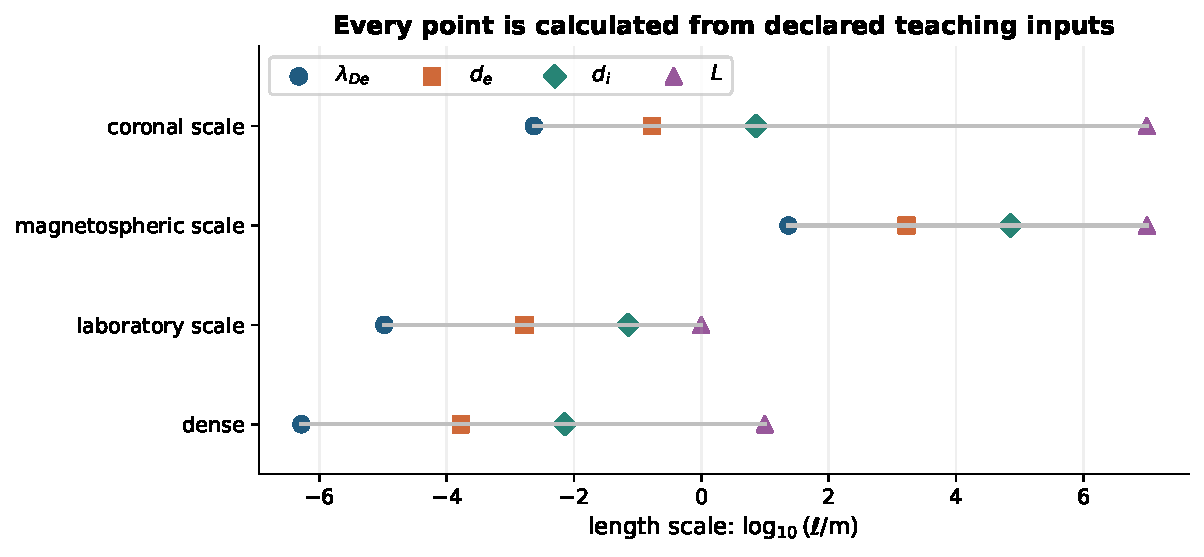
\includegraphics[width=.98\textwidth]{figures/03_scales.pdf}
\caption{四组教学输入对应的长度。横轴是米数的十进对数；间隔1代表长度相差10倍。$d_i/d_e$由质量比固定，而$L/d_i$与$\lambda_{De}/d_e$依参数改变。}\label{hall:figscales}\end{figure}

\subsection{例一：把实验室量级的每一步真的代进去}
取$n=10^{19}\,\mathrm{m^{-3}}$、$B=0.05\,\mathrm T$、$T_i=T_e=20\,\mathrm{eV}$、$L=1\,\mathrm m$。先算质量密度
\begin{equation}
\rho\simeq nm_i=1.67262\times10^{-8}\,\mathrm{kg/m^3}.
\end{equation}
因此
\begin{align}
V_A&=\frac{0.05}{\sqrt{(1.25664\times10^{-6})(1.67262\times10^{-8})}}
=3.4488\times10^5\,\mathrm{m/s},\\
\Omega_i&=\frac{(1.60218\times10^{-19})(0.05)}{1.67262\times10^{-27}}
=4.7894\times10^6\,\mathrm{s^{-1}},\\
d_i&=V_A/\Omega_i=0.07201\,\mathrm m,\\
d_e&=0.07201/\sqrt{1836.15}=1.6805\times10^{-3}\,\mathrm m,\\
\lambda_{De}&=\sqrt{\frac{(8.85419\times10^{-12})(3.20435\times10^{-18})}
{(10^{19})(1.60218\times10^{-19})^2}}
=1.0513\times10^{-5}\,\mathrm m.
\end{align}
电子压强$p_e=n\Theta_e=32.0435\,\mathrm{Pa}$，磁压$B^2/(2\mu_0)=994.72\,\mathrm{Pa}$，故$\beta_e=0.03221$。离子热速度$6.190\times10^4\,\mathrm{m/s}$，所以$\rho_i=0.01292\,\mathrm m$；$\rho_s=0.009139\,\mathrm m$。本例$d_i$约7.2厘米，而$\rho_i$约1.3厘米，二者不可互换。

密度换算为$10^{13}\,\mathrm{cm^{-3}}$后，
\begin{align}
\nu_{ei}&\simeq2.91\times10^{-6}\frac{10^{13}\times10}{20^{3/2}}
\simeq3.25\times10^6\,\mathrm{s^{-1}},\\
\eta_D&=\frac{(9.1094\times10^{-31})(3.2494\times10^6)}{(10^{19})(1.60218\times10^{-19})^2}
=1.1531\times10^{-5}\,\Omega\,\mathrm m,\\
D_\eta&=9.176\,\mathrm{m^2/s},\qquad
\lambda_{\rm mfp,e}=\frac{2.6524\times10^6}{3.2494\times10^6}=0.8163\,\mathrm m.
\end{align}
结果告诉我们：虽然有碰撞，电子沿温度变化长度的局地输运近似仍可能不成立；若沿场长度只有厘米，平均自由程明显更长。不能用“$\nu_{ei}$看起来很大”替代无量纲比较。

\subsection{例二：同一组参数，不同层厚得到不同模型}
取参考场$E_A=V_AB=1.7244\times10^4\,\mathrm{V/m}$，并暂取$\ell_B=\ell_p=\ell$。这是比较特征幅度，不是在X点把$U\times B$当作实际非零项。下表全部来自刚才的输入：
\begin{longtable}{P{29mm}rrrr}
\toprule 层厚$\ell$ & $1\,\mathrm m$ & $0.10\,\mathrm m$ & $0.010\,\mathrm m$ & $d_e=1.68\,\mathrm{mm}$\\\midrule
$E_H/E_A$ &0.0720&0.720&7.20&42.85\\
$E_p/E_A$ &0.00116&0.0116&0.116&0.690\\
$E_\eta/E_A$ &$2.66\times10^{-5}$&$2.66\times10^{-4}$&$2.66\times10^{-3}$&0.0158\\
$E_{m_e}/E_H$ &$2.82\times10^{-6}$&$2.82\times10^{-4}$&0.0282&1.00\\\bottomrule
\end{longtable}
最后一行分母是$E_H$，前三行分母是$E_A$，不能把四行直接相加。若要得到惯性相对$E_A$，应乘上第一行，例如$\ell=1$厘米时为$0.0282\times7.20=0.203$。到了$d_e$，忽略电子惯性的排序已经失败，不能继续用质量小作为理由。

在$\ell=0.1$米处，具体电场幅度为
\begin{align}
E_H&\sim0.720E_A=1.24\times10^4\,\mathrm{V/m},\\
E_p&\sim\Theta_e/(e\ell)=20/0.1=200\,\mathrm{V/m},\\
E_\eta&\sim\eta_D B/(\mu_0\ell)=4.59\,\mathrm{V/m}.
\end{align}
若该区域离子入流仅$0.1V_A$，对应的对流电场是$1.724\times10^3\,\mathrm{V/m}$，Hall幅度比值又大10倍。但真正要判断$E_z$时，必须用$(J_xB_y-J_yB_x)/(en)$，不能把$|J||B|/(en)$无条件塞给$z$分量。
\begin{figure}[htbp]\centering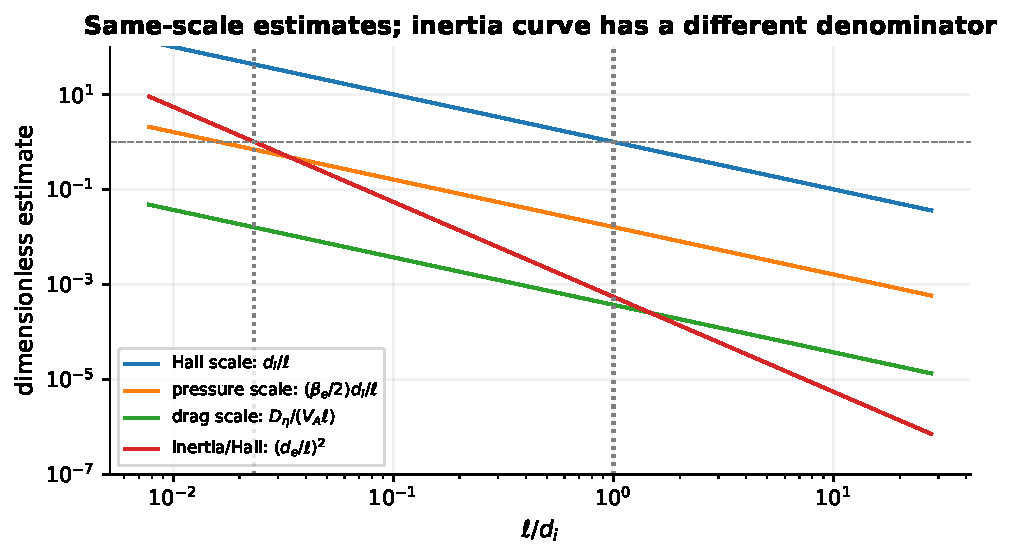
\includegraphics[width=.98\textwidth]{figures/04_ordering.pdf}
\caption{实验室教学参数下的同尺度估计。惯性曲线特意标明分母为Hall量级；其他三条除以$V_AB$。这些曲线表示排序如何随层厚改变，不是任何一次模拟的实测欧姆定律分解。}\label{hall:figordering}\end{figure}

\subsection{例三：为什么准中性成立而电子惯性仍要保留}
仍取实验室例，但$\ell=d_e=1.6805$毫米。假定$e\phi\sim\Theta_e$，电荷差相对密度为
\begin{equation}
\left(\frac{1.0513\times10^{-5}}{1.6805\times10^{-3}}\right)^2
=3.91\times10^{-5}.
\end{equation}
它很小，而$(d_e/\ell)^2=1$。因此\emph{准中性并不排除电子惯性}。若用Alfvén速度估计位移电流，其比值$(V_A/c)^2=1.32\times10^{-6}$。但电子流若达到电子Alfvén速度$V_{Ae}=V_A\sqrt{m_i/m_e}=1.478\times10^7\,\mathrm{m/s}$，相应估计上升至$2.43\times10^{-3}$；仍小，却不是前一个数。还应检查实际时间频率相对$\omega_{pe}$。

\subsection{例四：磁层不是把实验室的厘米改写成千米}
取$n=10^7\,\mathrm{m^{-3}}=10\,\mathrm{cm^{-3}}$、$B=20$ nT、$T_e=100$ eV、$T_i=1000$ eV。得到$V_A=138$ km/s、$d_i=72.0$ km、$d_e=1.68$ km、$\lambda_{De}=23.5$ m。离子$\beta_i=10.1$，所以
\begin{equation}
\rho_i=d_i\sqrt{\beta_i}=72.0\times\sqrt{10.1}\simeq228\,\mathrm{km}.
\end{equation}
如果层厚100 km，$d_i/\ell=0.720$，但$\rho_i/\ell=2.28$；Hall与离子有限轨道宽度都不能忽视。电子惯性/Hall约为$(1.68/100)^2=2.82\times10^{-4}$，暂小；电子压强量级/Hall约为$\beta_e/2=0.503$，已经不小。

$\nu_{ei}=5.81\times10^{-7}\,\mathrm{s^{-1}}$、$L/V_A=72.5$秒，所以$\nu_{ei}\tau_A=4.21\times10^{-5}$。沿系统通过的时间内，库仑碰撞极少；由此计算出的经典电阻只能作为很小的参照，不能把它当成已经证明能负责破冻结的机制。

\subsection{例五：强导场下必须分清哪个磁场进入哪个尺度}
在实验室例中保留反向分量$B_r=0.05$ T，另加$B_g=0.50$ T。重联可释放的反向场能量和对应$V_{Ar}$仍用$B_r$；回旋运动感受到的总场约$0.5025$ T。因此回旋半径约缩小为原来的$0.05/0.5025=0.0995$倍：$\rho_i\simeq1.286$毫米，$\rho_s\simeq0.909$毫米；$d_i=72.0$毫米完全不变，因为惯性长度不含$B$。

若需要判断强导场下的离子声/有限回旋效应，$\rho_s$可能比$d_i$更相关；若需要估计由反向场梯度形成的电流，分子仍是$B_r$。这一步明确后，才谈“Hall尺度由哪一个长度控制”；不能只替换一个符号便声称所有反平行结论都成立。

\section{例六：改变电子质量会具体改变什么}
很多计算把$m_i/m_e$从1836改成100或25以降低成本。在$n,B,m_i$固定时，$d_i,V_A,\Omega_i$不变，而$d_e/d_i$依次为0.02334、0.10、0.20。若每个$d_e$用8格，$100d_i$宽的方向所需格数为
\begin{align}
N_{1836}&=100d_i/(d_e/8)=34280,\\
N_{100}&=8000,\qquad N_{25}=4000.
\end{align}
二维格数约按一维格数平方增长，三维更昂贵。这解释了缩质量比的动力。但电子热速度、惯性响应、$\Omega_e$以及两个层的分离都随之改变；它不只是把计算钟变快。应至少比较一组质量比序列，并固定清楚物理或无量纲输入，不能把缩质量比的一张温图当成真实质量比结论。

\chapter{把方程放回重联层：Sweet--Parker、Hall层与电子层}
\label{hall:reconnection}
\section{为什么重联需要同时考虑入口与出口}
考虑稳态二维矩形扩散区，半长$L$，半厚$\delta$。上下两面入流，左右两面出流。若两侧对称，每单位$z$长度的质量通量是
\begin{equation}
2(2L)\rho_{\rm in}v_{\rm in}=2(2\delta)\rho_{\rm out}v_{\rm out}.
\end{equation}
每边都含两面和全长，约掉4，得到
\begin{equation}\rho_{\rm in}v_{\rm in}L=\rho_{\rm out}v_{\rm out}\delta.\end{equation}
若密度近似不变，再有$v_{\rm in}/v_{\rm out}=\delta/L$。因此长而窄的通道无法同时承载很大的入口质量通量和有限的出口速度；这不是电阻本身的结论，而是几何和质量守恒的约束。

磁张力将等离子体加速向外。按单位体积动量估计，惯性$\rho v_{\rm out}^2/L$与磁张力$B^2/(\mu_0L)$平衡，故
\begin{equation}v_{\rm out}\sim B/\sqrt{\mu_0\rho}=V_A.\end{equation}
这是假定下游背压、黏性、流剪切及其他能量损失没有强烈降低出流的量级关系，不是每个位置速度都恰好等于$V_A$。

\section{Sweet--Parker的三个条件如何一步步消元}
稳态二维Faraday定律要求$\partial_xE_z=\partial_yE_z=0$，故同一个$E_z$贯穿上游和扩散区。上游近理想，有$|E_z|\simeq v_{\rm in}B$；片心反向场很小，电阻模型给$|E_z|\simeq\eta|J_z|$。用$|J_z|\sim B/(\mu_0\delta)$，依次得到
\begin{align}
v_{\rm in}B&\sim\eta\frac{B}{\mu_0\delta},\\
v_{\rm in}&\sim\frac{D_\eta}{\delta}.
\end{align}
与连续性$v_{\rm in}\sim V_A\delta/L$相等：
\begin{align}
\frac{D_\eta}{\delta}&\sim\frac{V_A\delta}{L},\\
\delta^2&\sim\frac{D_\eta L}{V_A},\\
\boxed{\frac{\delta_{SP}}L\sim S_L^{-1/2}},\qquad
\boxed{\frac{v_{\rm in}}{V_A}\sim S_L^{-1/2}},\qquad S_L&=\frac{LV_A}{D_\eta}.
\end{align}
三个条件是质量通量、Alfvén量级出流和电场匹配。单独看欧姆定律无法决定$L$或$\delta$；把层长任意缩短，当然能得到更大速率，但那不是对层长选择的解释。

\worked{高密度教学例：一个较接近电阻MHD排序的情况}
用前章高密度例$L=10$ m、$V_A=3.4488\times10^4$ m/s、$D_\eta=51.386$ m$^2$/s，算得
\begin{align}
S_L&=\frac{10\times3.4488\times10^4}{51.386}=6.71\times10^3,\\
\delta_{SP}&=\frac{10}{\sqrt{6711.5}}=0.1221\,\mathrm m,\\
v_{\rm in}&=\frac{3.4488\times10^4}{\sqrt{6711.5}}=421\,\mathrm{m/s},\\
E_z&\sim v_{\rm in}B=21.0\,\mathrm{V/m}.
\end{align}
此时$d_i/\delta_{SP}=0.0590$、$\rho_i/\delta_{SP}=0.0529$、$\lambda_{\rm mfp,e}/\delta_{SP}=0.00597$。对于粗略的层结构，Hall和离子轨道尺度较小，碰撞局地性也更合理。它仍不是一个已证明稳定的实验解：大尺度稳定性、黏性和其他输运需要另查。

\worked{实验室教学例：全局MHD看似合理，内层却失败}
$S_L=3.7585\times10^4$、$\delta_{SP}=5.158$毫米、$v_{\rm in}=1.779$ km/s、$E_z=88.95$ V/m。核对电阻一侧：
\begin{equation}
J\sim\frac{0.05}{(1.25664\times10^{-6})(0.005158)}=7.71\times10^6\,\mathrm{A/m^2},
\quad \eta_DJ=88.95\,\mathrm{V/m}.
\end{equation}
数值匹配得很好，但$d_i/\delta_{SP}=13.96$、$\rho_i/\delta_{SP}=2.51$、$\lambda_{\rm mfp,e}/\delta_{SP}=158$。离子尺度比较已说明\textbf{我们解对了一个不适用的单流体经典电阻层模型}。平均自由程应与有关轨道方向、尤其平行方向的梯度尺度比较；此处与横向片厚的比值仅作警报，不能单独否定经典电阻闭合。代数自洽不等于物理自洽；下一步应检查双流体、压力张量和非局地闭合，而不是把这5毫米直接当预测。

\section{从一个不等式判断何时需要重新审查模型}
将$\delta_{SP}\lesssim d_i$代入上式：
\begin{align}
LS_L^{-1/2}&\lesssim d_i,\\
S_L^{1/2}&\gtrsim L/d_i,\\
\boxed{S_L\gtrsim(L/d_i)^2}.\label{hall:spthreshold}
\end{align}
这是反平行、该经典层宽估计下的\emph{自洽性警报}，不是普适Hall启动充分条件。系统是否到达该层宽、是否先发生撕裂/磁岛、是否强导场、边界怎样供磁、是否有迟滞，都能改变实际演化。\citep{Cassak2005,Ng2015}
\begin{figure}[htbp]\centering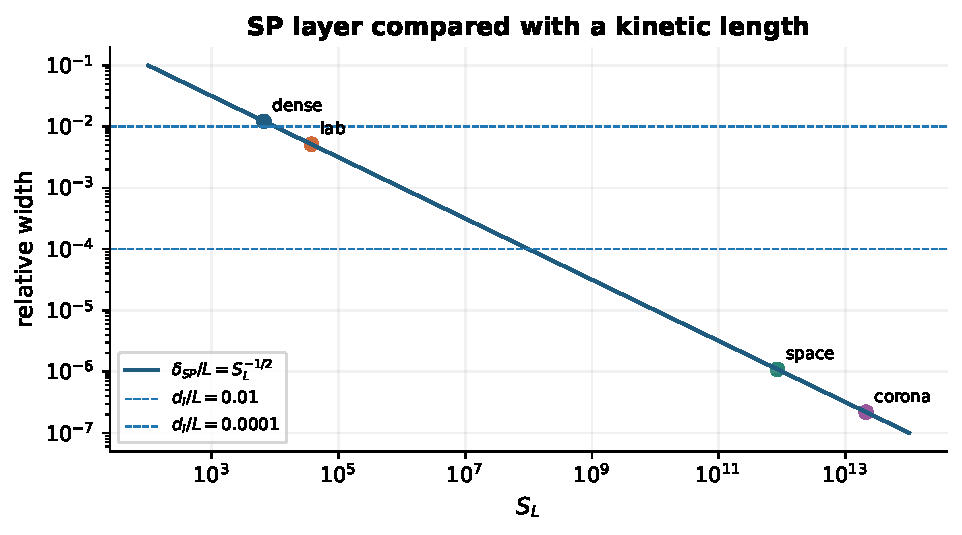
\includegraphics[width=.95\textwidth]{figures/07_sp.pdf}
\caption{Sweet--Parker层厚解析标度与固定$d_i/L$的比较。交点对应式\eqref{hall:spthreshold}；四个点来自教学参数。曲线不表示所有大$S$系统都能保持单一稳态长片。}\label{hall:figsp}\end{figure}

日冕教学例$L=10^7$ m、$V_A=3.4488\times10^6$ m/s给$S_L=2.10\times10^{13}$，经典层厚$2.182$ m，而$d_i=7.201$ m，比例$\delta_{SP}/d_i=0.303$。跨整个系统的Alfvén时间为2.90秒，按该单片SP入口速度处理系统磁通的时间为
\begin{equation}
\tau_{\rm SP}\sim\frac{L}{v_{\rm in}}=\tau_A\sqrt{S_L}
=1.33\times10^7\,\mathrm s\simeq154\,\text{天}.
\end{equation}
这个漫长时间只是该组输入与单片模型的结果，不是在模拟真实日冕事件。且$\lambda_{\rm mfp,e}\sim102$ km远大于2.18米，需要进一步核对粒子轨道和平行梯度的局地性，不能仅凭横向片厚判定碰撞闭合失效。实验室例与日冕例分别有$\nu_{ei}\tau_A=9.42$和168.5，它们也不是系统尺度上的完全无碰撞例。长片还可能先受撕裂不稳定性影响。应先改变模型或几何，不应把矛盾隐藏在一个调大电阻的参数里。

磁层教学例形式上给$\delta_{SP}=10.9$ m，甚至小于$\lambda_{De}=23.5$ m，也远小于$d_e=1680$ m。至此，使用准中性单流体经典SP层的多项排序一起失败；不能将这个数当作实际电子扩散区宽度。

\section{Hall层怎样改变流动，又为什么仍需要电子层}
在$d_e\ll\ell\lesssim d_i$的适用条件下，电子常仍保持近似磁化，而离子对局地电磁结构不能像大尺度那样即时响应。由于$\vct u_e=\vct u_i-\J/(en)$，磁通的运动可以接近电子流，离子质量通量的运动却与它不同。用一个共同速度和一个共同出口宽度的SP几何不再充分。

这种分离能够重排磁张力、面内电场、流入/排出通道及磁通输运，因而改变整体重联过程。但是取正压关系$p_e=p_e(n)$，并把电子电阻、惯性及非标量压力项删除后，
\begin{equation}
\E+\vct u_e\times\B=-\nabla h_e
\end{equation}
仍给出电子磁通冻结（若$h_e$是单值标量）。Hall项让磁场不再随\emph{离子}冻结，却未自动解除随\emph{电子}的冻结。有限电阻、非对角电子压力、电子惯性或明确的其他机制必须在电子内层中承担非理想作用。数值耗散也能做到，但必须诚实标明它是数值断线机制。\citep{Birn2001,Shay2001,Wang2015}

\section{为什么会出现四极面外磁场：用安培定律读图}
取二维$\partial_z=0$，面外场$B_z(x,y)$与面内电流满足
\begin{equation}
J_x=\frac{1}{\mu_0}\partial_yB_z,\qquad
J_y=-\frac{1}{\mu_0}\partial_xB_z.
\end{equation}
电子和离子的面内流不同，形成闭合的面内电流路径；这些电流会产生具有不同象限极性的$B_z$。反过来，测得二维$B_z$梯度可以推断面内电流。图\ref{hall:figquad}用一个显式解析函数检验此关系，既没有声称满足完整重联方程，也没有把电流线说成磁力线。
\begin{figure}[htbp]\centering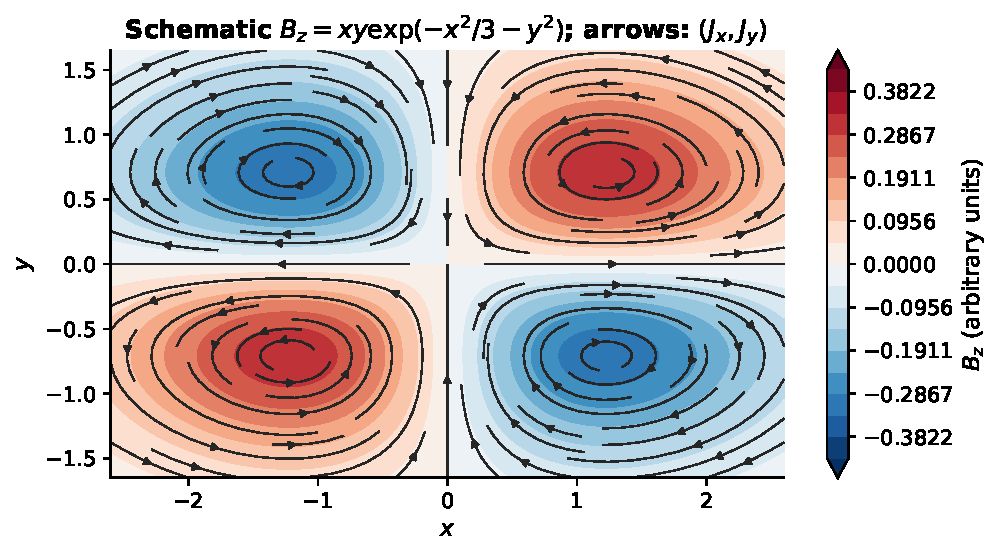
\includegraphics[width=.97\textwidth]{figures/05_quadrupole.pdf}
\caption{四极场与面内电流的教学示意。色彩是$B_z=xy\exp(-x^2/3-y^2)$，黑箭头严格由$J_x\propto\partial_yB_z,J_y\propto-\partial_xB_z$生成。颜色表示场的面外正负，箭头表示电流，二者不是同一种矢量。整体极性依反向场、坐标和电流方向改变。}\label{hall:figquad}\end{figure}

四极图样是重要线索，却不是“所有Hall预测已验证”的充分证据。导场、非对称、额外物种、三维结构和多个X点能使图样变形。要结合电子/离子流、电场分量和尺度判断。特别是反平行二维X点$\B=0$时，$\J\times\B=0$：\emph{旁边看到很强Hall场，并不能用它在零场X点直接支撑$E_z$。}

\section{重联率怎样从磁通计算}
在二维$A_z$约定下，$E_z=-\partial_tA_z$（取$\partial_z\phi=0$）。设X、O点位置都随时间变化，对磁通差作全导数：
\begin{align}
\frac{\dd}{\dd t}[A_z(O,t)-A_z(X,t)]
&=\partial_tA_z|_O+\dot{\vct x}_O\cdot\nabla A_z|_O
-\partial_tA_z|_X-\dot{\vct x}_X\cdot\nabla A_z|_X\\
&=E_z(X)-E_z(O).
\end{align}
第二步利用X和O都是$A_z$驻点，梯度为零。只有参考O点的$E_z$可忽略或已被适当扣除时，才将$E_z(X)$单独叫磁通变化率。归一率通常取$\mathcal R=E_{\rm rec}/(B_{\rm up}V_{A,\rm up})$；上游场、密度和位置要明确。若$B_{\rm up}$随时间改变，两个相同的归一率也可能对应不同的实际电压和功率。

\worked{速率不是功率，也不是温升}
取实验室例$B_{\rm up}=0.05$ T、$V_A=3.4488\times10^5$ m/s。若\emph{人为指定}某过程$\mathcal R=0.10$，则$E_{\rm rec}=1.7244\times10^3$ V/m。沿$z$长度0.2 m的均匀区，对应电动势约345 V。它只有与电流密度点乘、对体积积分后才成为功率；还需扣除边界Poynting通量、流能和热输运，才能讨论物种加热。这里的0.10是演示输入，不是由Hall方程独自推出来的普适常数。

\chapter{用一个能完整求解的波动问题理解Hall项}
\label{hall:waves}
\section{为什么重联讲义还要讲波}
波动是检验方程物理内容和数值实现的最小问题。Hall项含一个额外空间导数，因而短波会比长波表现出更强的双流体差异。我们不用一句“出现whistler所以重联快”替代推导，而是先把色散关系算出来，再讨论它能解释和不能解释的事。

取均匀静止平衡$n=n_0,\B=B_0\hat{\vct z}$，忽略压缩、压强扰动、电阻和电子惯性，仅考虑沿场传播的横向小扰动
\begin{equation}
\vct u=\vct u_1e^{i(kz-\omega t)},\qquad
\B=B_0\hat{\vct z}+\vct b_1e^{i(kz-\omega t)},\qquad
u_{1z}=b_{1z}=0.
\end{equation}
实物理量取复表达式的实部；$i$只记录相位。线性化时保留一阶扰动，把$\vct u_1\times\vct b_1$等二阶小量删除。

\section{逐项计算旋度与磁张力}
因为$\nabla=ik\hat{\vct z}$，
\begin{equation}
\J_1=\frac{ik}{\mu_0}\hat{\vct z}\times\vct b_1.
\end{equation}
再用$(\hat{\vct z}\times\vct b_1)\times\hat{\vct z}=\vct b_1$，得到
\begin{equation}
-i\omega\rho_0\vct u_1=\J_1\times B_0\hat{\vct z}
=\frac{ikB_0}{\mu_0}\vct b_1.
\end{equation}
两边除以$i$，注意左边负号，故
\begin{equation}\vct u_1=-\frac{kB_0}{\mu_0\rho_0\omega}\vct b_1.\label{hall:waveu}\end{equation}
对感应方程
\begin{equation}
\partial_t\B=\nabla\times(\vct u\times\B)
-\nabla\times\left(\frac{\J\times\B}{en_0}\right),
\end{equation}
第一项为$ikB_0\vct u_1$；第二项为
\begin{align}
-ik\hat{\vct z}\times\left(\frac{ikB_0}{\mu_0en_0}\vct b_1\right)
&=\frac{k^2B_0}{\mu_0en_0}\hat{\vct z}\times\vct b_1,
\end{align}
因为$-i^2=+1$。令$C_H=B_0/(\mu_0en_0)=V_Ad_i$，则
\begin{equation}
-i\omega\vct b_1=ikB_0\vct u_1+C_Hk^2\hat{\vct z}\times\vct b_1.\label{hall:waveb}
\end{equation}
$C_H$单位是$\mathrm{m^2/s}$，所以$C_Hk^2$确为频率。

\section{圆偏振把矢量问题化成一个二次方程}
选择$\vct b_1=b(\hat{\vct x}+i\sigma\hat{\vct y})$，$\sigma=\pm1$。直接相乘可验
\begin{equation}
\hat{\vct z}\times\vct b_1=b(\hat{\vct y}-i\sigma\hat{\vct x})=-i\sigma\vct b_1.
\end{equation}
代入式\eqref{hall:waveb}并除以$-i$：
\begin{equation}\omega\vct b_1=-kB_0\vct u_1+\sigma C_Hk^2\vct b_1.\end{equation}
再代入式\eqref{hall:waveu}，消去$\vct u_1$：
\begin{align}
\omega&=\frac{k^2B_0^2}{\mu_0\rho_0\omega}+\sigma C_Hk^2,\\
\boxed{\omega^2-\sigma k^2V_Ad_i\omega-k^2V_A^2=0}.
\end{align}
取$k>0$，两支正频率为
\begin{equation}
\boxed{\omega_\pm=\frac{kV_A}{2}\left[\sqrt{4+k^2d_i^2}\pm kd_i\right]}.
\end{equation}
两支分别属于两种圆偏振；负频率解与相反传播/偏振的表示有关，不额外创造新的正能量分支。

令$x=kd_i$并用$V_A/d_i=\Omega_i$，则
\begin{equation}
\frac{\omega_\pm}{\Omega_i}=\frac{x}{2}\left(\sqrt{4+x^2}\pm x\right).
\end{equation}
$x\ll1$时，$\sqrt{4+x^2}=2+x^2/4+\cdots$，所以两支都趋向$kV_A$；$x\gg1$时，用$\sqrt{x^2+4}=x+2/x+\cdots$，得到
\begin{equation}
\omega_+\simeq k^2V_Ad_i,\qquad \omega_-\simeq V_A/d_i=\Omega_i.
\end{equation}
前者是whistler支，后者趋近离子回旋频率。在真实温等离子体中，有限回旋半径、共振和阻尼会进一步改变它们；这里是冷、平行、无耗散Hall极限。
\begin{figure}[htbp]\centering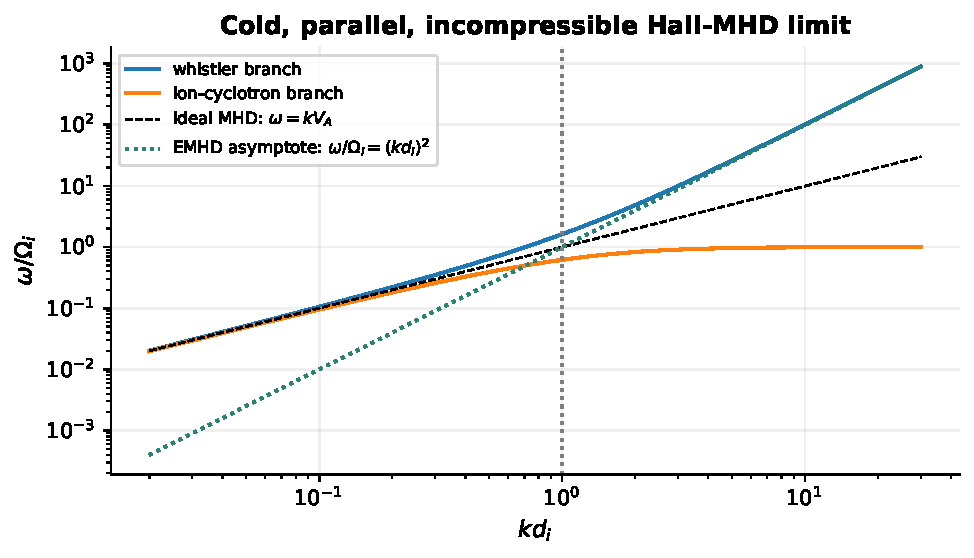
\includegraphics[width=.96\textwidth]{figures/06_dispersion.pdf}
\caption{由本章二次方程直接计算的两支色散关系，不是数值模拟拟合。$kd_i\ll1$时回到MHD；短波whistler频率随$k^2$增长，提示显式时间步会随网格变细而更严格。}\label{hall:figwave}\end{figure}

\worked{波长、波数和频率的完整换算}
仍取实验室教学参数。$d_i=0.072008$ m、$\Omega_i=4.7894\times10^6$ s$^{-1}$。
当$kd_i=0.1$时，$k=1.3887$ m$^{-1}$，$\lambda=2\pi/k=4.525$ m。两支$\omega_+/\Omega_i=0.105125$、$\omega_-/\Omega_i=0.095125$，故普通频率分别为80.1 kHz、72.5 kHz。它们相近，但并不完全相等。

当$kd_i=1$时，$\lambda=0.4525$ m，两个比值分别为1.6180和0.6180，频率分别为1.233 MHz和0.471 MHz。当$kd_i=10$时，$\lambda=4.525$ cm，whistler比值为100.990，频率约77.0 MHz；此时$kd_e=0.2334$，电子惯性修正已经不再极小。不要把$d_i$叫“波长”：$k d_i=1$对应的是$\lambda=2\pi d_i$，差一个$2\pi$。

\section{电子惯性如何限制无界的短波增长}
若进一步取固定离子、常密度、不可压电子流，保留电子惯性，可定义
\begin{equation}\B_e=\B-d_e^2\nabla^2\B.\end{equation}
在线性平行扰动中$\nabla^2\vct b_1=-k^2\vct b_1$，所以$\vct b_e=(1+d_e^2k^2)\vct b_1$，固定离子的whistler色散关系变为
\begin{equation}
|\omega|=\frac{C_Hk^2}{1+d_e^2k^2},\qquad
\lim_{kd_e\to\infty}|\omega|=\frac{C_H}{d_e^2}=|\Omega_e|.
\end{equation}
这不是前面完整离子响应色散关系在所有$k$上的精确替代式，而是另一组已说明近似的电子流体极限。它说明电子惯性不会永远容许无质量Hall模型的$k^2$频率增长。

在$kd_e\ll1$的whistler区，$v_{\rm ph}=\omega/k=C_Hk$，$v_g=\dd\omega/\dd k=2C_Hk$。包含上述电子惯性后，
\begin{equation}v_g=\frac{2C_Hk}{(1+d_e^2k^2)^2}.\end{equation}
色散让不同尺度以不同速度传播，能够改变重联层的通讯和形态，但这一线性波公式并未求解非线性层长、边界供能或破冻结，所以不能单凭它推导所有重联率等于某个常数。

\chapter{从方程到模拟，再到实验：怎样判断一项结果可信}
\label{hall:practice}
\section{建立一个最小Hall算例前，先把未知量写全}
不要直接从一张好看的重联图开始。先声明模型，例如准中性氢、$m_e=0$、标量双温、无粒子源、给定电阻率、规定的热流和碰撞交换。演化$n,\vct u_i,p_i,p_e,\B$；由$\J=\nabla\times\B/\mu_0$和$\vct u_e=\vct u_i-\J/(en)$得到电子速度。欧姆定律给$\E$，Faraday定律推进$\B$。电子压强应沿电子流对流，不能只是复制一份沿离子流的能量式。

完整初始化至少包括：密度、两温、磁场及$\nabla\cdot\B=0$；满足总压平衡的电流片；电流由两物种如何承担；扰动的磁通幅度和波数；周期/导体/开放边界；所有耗散与热源系数。周期边界意味着出流最终会回到计算域或遇到另一片，不是无限开放空间。加入有限磁岛种子可绕过线性撕裂阶段，不能再用启动时间声称自然触发机制已预测。

如果选择全Maxwell五矩/十矩，应分别推进两套$n_s,m_sn_s\vct u_s$和能量/压力，电场也有独立演化式；高频等离子体振荡和光波刚性随之出现。这个实现与准中性Hall的变量、约束和边界不相同，不能只在Hall代码里加一个电子动量项便自称完整Maxwell双流体。

\section{归一化不是隐藏单位：完整写出一套转换}
选择参考$n_0,B_0,L_0$，并定义
\begin{equation}
V_0=\frac{B_0}{\sqrt{\mu_0n_0m_i}},\quad
 t_0=\frac{L_0}{V_0},\quad J_0=\frac{B_0}{\mu_0L_0},\quad
E_0=V_0B_0,\quad p_0=\frac{B_0^2}{\mu_0}.
\end{equation}
这里$p_0$是磁压$B_0^2/(2\mu_0)$的两倍，选哪种都可以，但无量纲系数必须一致。令帽号表示除以对应参考量，欧姆定律为
\begin{equation}
\widehat{\E}+\widehat{\vct u}_i\times\widehat{\B}
=\frac{d_{i0}}{L_0}\frac{\widehat{\J}\times\widehat{\B}}{\widehat n}
-\frac{d_{i0}}{L_0}\frac{\widehat\nabla\widehat p_e}{\widehat n}
+\frac{1}{S_0}\widehat{\J},
\qquad S_0=\frac{\mu_0L_0V_0}{\eta}.
\end{equation}
压强若改用$n_0\Theta_{e0}$归一化，压力项前还需出现$\beta_{e0}/2$。不能在归一化后忘记它原来藏在压强定义里。

\worked{读取无量纲模拟输出}
取前文实验室例并选择$L_0=d_i=0.072008$ m，则$t_0=d_i/V_A=2.088\times10^{-7}$ s，也就是$\Omega_i^{-1}$。若代码输出$t=50$、电场$E_z=0.08$、位置$x=10$，其物理值为10.44微秒、1379.5 V/m、0.7201 m。若输出$p_e=0.0161$，乘$p_0=1989.4$ Pa得到32.0 Pa；这与$\beta_e=0.0322$相符。归一化温度还必须用$p/n$换回，不能把无量纲$p$直接叫eV。

\section{网格为什么被电子尺度和Hall波限制}
空间分辨率应该由所声称的最窄物理结构决定。若要分辨$d_e$内层而只用$\Delta x=0.5d_e$，只有两格，通常不足以支持其厚度与峰值的精确结论。所谓每尺度8格也只是起点；需比较更细网格并检查实际观测量。

无质量Hall的短波频率约$\omega\sim C_Hk^2$。若取最高网格波数$k_{\max}\sim\pi/\Delta x$，显式时间积分至少需$\omega_{\max}\Delta t$在其稳定域内，因此
\begin{equation}\Delta t_H\lesssim C_{\rm time}\frac{\Delta x^2}{C_H},\end{equation}
$C_{\rm time}$依空间离散及时间积分器决定，不能作为普适常数。它比通常的对流$\Delta t\propto\Delta x$更苛刻；网格缩小一半，Hall时间步常要缩小到约四分之一。电阻扩散同样给$\Delta t\propto\Delta x^2/D_\eta$。

\worked{一个时间步数量级例子}
实验室例$C_H=V_Ad_i=2.483\times10^4$ m$^2$/s。取$\Delta x=0.5$毫米，用粗略$C_{\rm time}=0.1$作\emph{教学估计}，
\begin{equation}\Delta t_H\sim0.1\frac{(5\times10^{-4})^2}{2.483\times10^4}=1.01\times10^{-12}\,\mathrm s.\end{equation}
这相当严苛，而$\Delta x<d_e$时无质量电子模型也正在丢失物理排序。隐式/半隐式推进可以缓解稳定性限制，但并不自动给出足够的时间精度或正确的电子闭合。若推进全Maxwell，光波条件约$\Delta x/c=1.67\times10^{-12}$ s，电子等离子体频率又引入额外时间尺度；选择约化模型是一项物理和数值的共同决定。

\section{用哪些检查排除“算得像”}
最小检查应同时包含：线性波频率与解析式一致；静态Harris平衡没有无故爆发；$\nabla\cdot\B$受控；总能预算包含边界通量；网格和时间步改小后，磁通率、层宽、峰值压力及积分能量趋于稳定。若使用压强下限、密度下限或限制器，它们改变的质量和能量必须记账。

建议把“数值误差”和“物理闭合差异”分开：先固定闭合做收敛，再在相同初边值下换闭合。两个模型若用不同质量比、不同种子和不同边界，差异不能唯一归因于Hall项。比较相同时间和相同重联磁通的图各有意义；前者比较时序，后者比较相近拓扑状态。论文若在不同时间取图，必须明确。

\section{GEM基准告诉了我们什么，也没有告诉什么}
Birn等的GEM挑战用规定的Harris片和有限磁岛种子比较MHD、Hall、混合与PIC。其主设置包括质量比25、背景密度为片心参考密度的0.2、片半厚0.5$d_i$、盒$25.6d_i\times12.8d_i$。含Hall响应的多类模型在该问题中的重联磁通曲线相近，传统小均匀电阻MHD则慢得多。\citep{Birn2001}

这支持Hall尺度的物种分离对该类非线性重联的重要性，但不是一条“只加Hall就解决一切”的定理。有限种子有意避开自然线性触发；各代码的电子惯性、压力及耗散实现并不完全相同；电子层和离子喷流的宽度仍可能相差约两倍。Shay等后继比较还显示密度空洞与喷流峰值存在明显模型差异。\citep{Shay2001}

因此学习顺序应是：先能重现基准的定义和输入，再检查不止一个输出，最后才扩大到导场、非对称、三维或装置几何。这里引用已有原文证据；本次讲义没有重新运行GEM的大规模模拟。

\section{实验例：MRX怎样把Hall效应变成可测量问题}
Ren等在MRX的氢/氘、无净初始导场重联中，用磁探针数组测量面外磁场。71通道高分辨率径向阵列间距1.25毫米，报告系统误差小于10 G；另有90通道二维阵列和用于重联场的29通道阵列。二维图通过径向扫描并合并多个放电构成，不是整个平面的单次同时高分辨率成像。\citep{Ren2005}

高分辨率测得的四极场幅度约50--60 G，相比约100 G的肩部重联场并不小。较粗二维图约20--40 G，原文把较小幅度与空间分辨率联系起来。四极结构横向尺度约为$d_i$，沿出流方向约为数个$d_i$。这些是空间结构、极性和尺度的共同证据。

\worked{把原文Hall电场估计重算一次}
原文采用$B_H\sim40$ G$=0.004$ T、四极场沿出流的峰间长度$L_H\sim18$ cm，用半长0.09 m估梯度：
\begin{align}
J_R&\sim\frac{0.004}{(1.25664\times10^{-6})(0.09)}
=3.54\times10^4\,\mathrm{A/m^2},\\
\frac{J_RB_Z}{en}&\sim
\frac{(3.54\times10^4)(0.020)}{(1.60218\times10^{-19})(3\times10^{19})}
=147\,\mathrm{V/m}.
\end{align}
这与原文约140 V/m的量级及典型约100 V/m的重联电场相当。但它取的是\emph{指定上游区域的指定分量}，并不证明X点处Hall项断线，也没有完整闭合所有欧姆项。原文指出部分区域的另一个磁场分量不够准确，尚不能全面评价。

其随碰撞性的扫描中，$B_H/B_{\rm rec}$约从0.6降至0.25，同时碰撞指标$\delta/\lambda_{\rm mfp}$从约0.2升至20；误差棒来自放电差异。它支持Hall结构与较弱碰撞条件的关联，但不能排除同时存在的波动或其他耗散。推断电子流还用到了电流主要由电子承担的假设，不能改写为直接测到了完整电子速度分布。原文图1--4及式(1)是建议带着本章公式阅读的定位。

\section{读论文的一个可重复流程}
按下面顺序读，会比先看“重联率接近0.1”的结论更有效：先抄出模型的独立变量和电子破冻结项；再抄归一化、质量比、导场与尺度；第三步检查边界、种子和耗散；第四步分别读取磁通率、压力、电场分量及能量预算；最后检查实验诊断和误差。未报告的网格或热源分配不要自行补上。对初学者，能明确说出“这张图不能推出什么”也是掌握模型的标志。

\chapter{完整解答：用十一道问题检查是否学会}
\label{hall:solutions}
本章不是把关键任务转交给读者。每题都给出解答，可以先遮住答案尝试，再逐行核对。

\section{密度相等，为什么还会有电流}
\textbf{题目：}$n_i=n_e=10^{19}$ m$^{-3}$，$u_{ix}=2\times10^4$ m/s，$u_{ex}=-3\times10^4$ m/s，求电荷密度与电流。

\textbf{解：}$\rho_c=e(n_i-n_e)=0$；$J_x=en(u_{ix}-u_{ex})=(1.60218\times10^{-19})(10^{19})(5\times10^4)=8.01\times10^4$ A/m$^2$。电荷密度是两个\emph{数密度}的差，电流是两个\emph{带符号电荷通量}的和。准中性没有要求两个流速相等。

\section{用质心和电流恢复两物种速度}
\textbf{题目：}$m_i/m_e=1836$，$\vct u=0$，$J_z/(en)=10^6$ m/s。

\textbf{解：}解$\vct u=(m_i\vct u_i+m_e\vct u_e)/(m_i+m_e)$与$\vct u_i-\vct u_e=\J/(en)$，得到
\begin{equation}
u_{iz}=\frac{m_e}{m_i+m_e}10^6=544.4\,\mathrm{m/s},\qquad
u_{ez}=-\frac{m_i}{m_i+m_e}10^6=-9.9946\times10^5\,\mathrm{m/s}.
\end{equation}
质心不动不等于粒子不动，也不等于流能为零；此时全部流能都属于两物种的相对漂移。

\section{Hall总功为零，但物种功可以不为零}
\textbf{题目：}$\J=J\hat{\vct z}$、$\B=B\hat{\vct x}$、$u_{iy}=U$，其余速度满足准中性电流关系。求Hall电场和两物种功。

\textbf{解：}$\hat{\vct z}\times\hat{\vct x}=\hat{\vct y}$，故$\E_H=JB\hat{\vct y}/(en)$。因为电流只有$z$分量，$u_{ey}=u_{iy}=U$。离子功$en\vct u_i\cdot\E_H=UJB$，电子功$-en\vct u_e\cdot\E_H=-UJB$，和为零。取$J=10^5$ A/m$^2$、$B=0.02$ T、$U=10^4$ m/s，两者为$\pm2\times10^7$ W/m$^3$。这是欧姆分解中特定电场分量的能量交换，不是两个必然为正的热源。

\section{同样大的压力电场，为什么未必改变磁通}
\textbf{题目：}恒温电子$\Theta_e$不变，$p_e=n\Theta_e$，写出压力项并求旋度。

\textbf{解：}
\begin{equation}
-\frac{\nabla p_e}{en}=-\frac{\Theta_e}{e}\frac{\nabla n}{n}
=-\nabla\left(\frac{\Theta_e}{e}\ln(n/n_\star)\right).
\end{equation}
这里$n_\star$是任意常数参考密度，使对数的自变量无量纲。在光滑单值区域，其旋度为零。它仍可平衡电子压力力、产生电势并改变粒子运动；只是不能单独在Faraday定律中提供感应源。若$\Theta_e$有独立空间梯度，旋度中出现$\nabla\Theta_e\times\nabla n$，必须重新计算。

\section{压缩升温是否就是不可逆加热}
\textbf{题目：}理想单原子标量流体绝热压缩，密度变为原来的2倍，温度变化多少？

\textbf{解：}无热流/耗散时$p/n^{\gamma_s}$沿流不变，$\gamma_s=5/3$。因为$\Theta=p/n$，所以$\Theta/\Theta_0=(n/n_0)^{\gamma_s-1}=2^{2/3}=1.5874$。20 eV升为31.75 eV。理想反向膨胀能回到20 eV，因此这次温升不必伴随熵增加。若要说不可逆，需检查碰撞、黏性、闭合熵或明确粗粒化的贡献。

\section{双束二阶矩为什么容易被叫成“热”}
\textbf{题目：}同一物种有两束各占一半，平均速度为$\pm U\hat{\vct x}$，每束内部各向同性温度能量为$\Theta_0$。求总流、压力和标量温度。

\textbf{解：}总流为零。按中心矩相加，$P_{xx}=n\Theta_0+nmU^2$，$P_{yy}=P_{zz}=n\Theta_0$。因此
\begin{equation}\Theta_{\rm moment}=\frac{\operatorname{tr}\vct P}{3n}=\Theta_0+\frac{mU^2}{3}.\end{equation}
对质子$U=100$ km/s，$m_iU^2/e=104.4$ eV，标量温度多出34.8 eV，但分布仍可保持两束，各束热宽并未增加。若只测$x$方向，额外的方向温度是104.4 eV。两种数不能混写。
\begin{figure}[htbp]\centering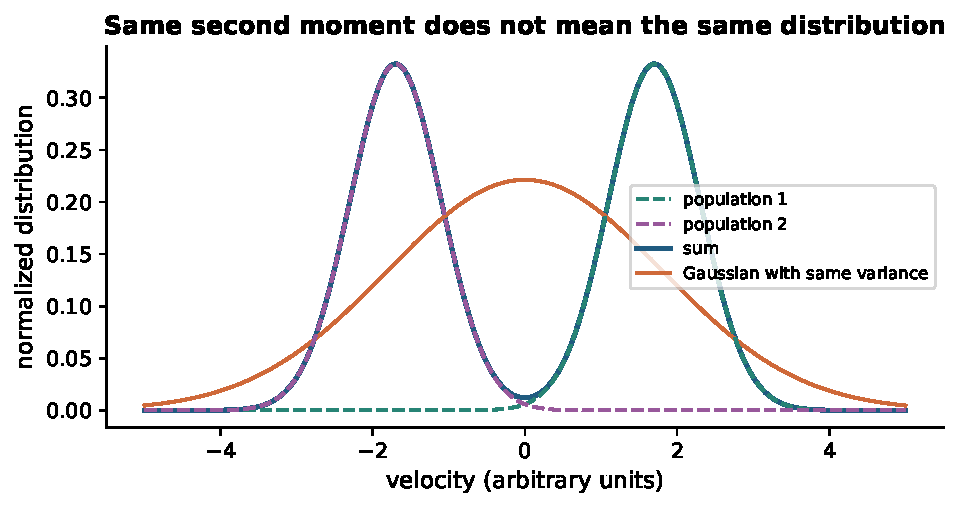
\includegraphics[width=.96\textwidth]{figures/08_multibeam.pdf}
\caption{两个窄高斯束及其和，与同二阶矩的单高斯对比。两者平均速度和方差可以相同，形状与分布熵却不同。图中参数是任意单位的教学输入，不是实验拟合。}\end{figure}

\section{局地各向同性化为什么不增加内能}
\textbf{题目：}只推进$\partial_t\vct P=-\nu(\vct P-p\vct I)$，$p=\operatorname{tr}\vct P/3$，初始$\vct P=\operatorname{diag}(4,1,1)$ Pa。求解。

\textbf{解：}取迹得到$\partial_t\operatorname{tr}\vct P=-\nu(\operatorname{tr}\vct P-3p)=0$，故$p=2$ Pa不变。分别解三个一阶方程：
\begin{equation}P_{xx}=2+2e^{-\nu t},\qquad P_{yy}=P_{zz}=2-e^{-\nu t}.\end{equation}
内能始终为$\operatorname{tr}\vct P/2=3$ J/m$^3$。压强越来越各向同性，不等于总内能越来越大；矩熵可因重排而增加，但要说明定义及闭合来源。

\section{网格缩小一半，Hall显式成本怎样变化}
\textbf{解：}二维格数约增加4倍，时间步若受Hall条件限制缩小为四分之一，同一物理时间需4倍步数，总基础计算量约增加16倍；三维格数增加8倍，总量约增加32倍。通信、隐式求解、缓存和并行效率会改变实际耗时，但这个估计足以说明为什么“再细一倍”不是小代价。仍不能因此省掉必要收敛检查。

\section{一次实验能否证明Hall在X点断线}
\textbf{题目：}二维反平行X点测到$E_z\ne0$，邻近区域测到四极$B_z$，是否可推出$E_z=(\J\times\B)_z/(en)$在X点成立？

\textbf{解：}不能。严格反平行零场X点$\B=0$，Hall项为零；若在二维对称强导场X点仅有$B_z$，$(\J\times\B)_z=J_xB_y-J_yB_x$也为零。非零$E_z$须由电子非理想项平衡。邻近Hall结构与电子内层破冻结是相互关联但不同的问题。

\section{给定密度和磁场，是否已经知道重联热量}
\textbf{解：}给定$B,n$可算每粒子参考磁能$B^2/(2\mu_0n)=m_iV_A^2/2$。实验室例为$6.21\times10^2$ eV每个离子--电子对的参考磁能量级。它没有告诉我们实际释放比例、向外输运比例、流能存储或两物种分配。即使假设全部变成两个物种的均匀标量内能，也只有
\begin{equation}\frac32(\Delta\Theta_i+\Delta\Theta_e)=\frac{B^2}{2\mu_0n},\end{equation}
一条式子约束两个未知温升。还需独立能量方程和机制，不能凭Hall项补一个固定2:1比例。

\section{一页自检：不用背诵，也应该能解释}
读完后应能连贯说明：Hall项来自电子--离子速度差；准中性允许有限电流；取矩是恒等操作而闭合是额外模型；电子惯性小不小取决于层厚、频率和速度；磁冻结应指明跟哪种速度；X点电场必须按分量检查；压力功、温升与不可逆热化不同；$d_i,\rho_i,\rho_s,\lambda_D$各有含义；一个全局大$S$不能保证局地MHD成立；一张四极图或一条相近重联率不足以证明闭合与加热全部正确。

如果其中某项仍只能复述结论，建议回到相应章节重算一个数字例。真正的掌握不是记住更多模型名字，而是能在新参数下重新选择近似，并明确模型预测的边界。

\backmatter\begingroup\small\setlength{\bibsep}{3pt}\bibliographystyle{unsrtnat}\bibliography{references}\endgroup
\end{document}
